\documentclass[pdfa,cucitura]{toptesi}

\hypersetup{
    pdfpagemode={UseOutlines},
    bookmarksopen,
    pdfstartview={FitH},
    colorlinks,
    linkcolor={blue},
    citecolor={red},
    urlcolor={blue}
}

%\linespread{1.3}

%
% Phantom space for abbreviations
%
\usepackage{xspace}
%
% To insert doi identifiers
%
\usepackage{doi}
\renewcommand{\doitext}{DOI }
%
% Improve citations from biblio
%
\usepackage{cite}
%
% This is to create hyperlinks for index, URLs and citations
% (now we can use the command \url{...} to create URL with hyperlink)
% 
%\usepackage{color}
%\usepackage[a4paper,colorlinks=true,urlcolor=blue,citecolor=blue,linkcolor=blue,bookmarks=false]{hyperref}
%
% For pasting text files
%
%\usepackage{fancyvrb}
%
% Used to express formulas like n^th
%
%\usepackage{mathtools}
%
% For table formatting
%
%\usepackage{longtable}
%\usepackage{makecell}
%\usepackage{multirow}
%
% For plotting results
%
%\usepackage{pgfplots}
%\pgfplotsset{compat=newest}
%
% For placing floats
%
%\usepackage{placeins}
%
% For subfigure environment
%
\usepackage{subcaption}
\usepackage{cleveref}
\captionsetup[subfigure]{subrefformat=simple,labelformat=simple}
\renewcommand\thesubfigure{(\alph{subfigure})}
%
% For Appendix section
%
%\usepackage[titletoc,toc,title]{appendix}
%
% Definition of margins
%
%\usepackage[top=2cm,bottom=2cm,left=2cm,right=2cm]{geometry}
%
% Paragraph skip and indent
%
%\setlength\parskip{\medskipamount}
%\setlength\parindent{0pt}
%
% For itemize and enumerate spacing
%
\usepackage{enumitem}
%
% For International System of Units (SI)
%
%\usepackage[binary-units]{siunitx}
%\sisetup{per-mode=symbol} % 1/s instead of s^-1
%
% For programming code
%
\usepackage{listings}
\lstset{
basicstyle=\ttfamily,
columns=fullflexible,
xleftmargin=3ex,
breaklines,
breakatwhitespace,
escapechar=`
}

% Some page parameters
\setlength{\parskip}{\medskipamount}
% Horizontal rule
\newcommand{\HRule}{\rule{\linewidth}{0.2mm}}


%
% Frequently used abbreviations.
% - example: \ie this is an example
%
\def\eg{e.g.\xspace}
\def\ie{i.e.\xspace}
\def\chap{Chapter\xspace}
\def\sec{Section\xspace}
\def\myfig#1{Fig.~#1\xspace} % usage: \myfig{\ref{fig:tag}}
\def\mytab#1{Tab.~#1\xspace}
\newcommand{\ltx}{\LaTeX\xspace}
\newcommand{\txw}{TeXworks\xspace}
\newcommand{\mik}{MikTex\xspace}
\newcommand{\html}{HTML\xspace}
\newcommand{\xhtml}{XHTML\xspace}
\newcommand{\cmd}[1]{\texttt{#1}\xspace}

% Styles
\newcommand{\itemname}{\textbf}
\newcommand{\thead}{\textbf}

% To cite RFC, es. \rfc{822}
\newcommand{\rfc}[1]{RFC-#1\xspace}
% To cite file (es. \file{autoexec.bat}) or fake URI (i.e. \file{http://www.lioy.it/})
% for real URIs use \url o \href
\newcommand{\file}[1]{\texttt{#1}\xspace}
% For inline code
\newcommand{\code}[1]{\lstinline|#1|}
% Backslash
\newcommand{\bs}{\textbackslash}
% Term definition with insertion into the index
\newcommand{\tdef}[1]{\textit{#1}\index{#1}}
% Meta-term
\newcommand{\meta}[1]{\textit{#1}}


\begin{document}
\selectlanguage{english}

\CorsoDiLaureaIn{Corso di Laurea Magistrale in }
\TesiDiLaurea{}
\AdvisorName{Supervisor}
\CandidateName{Candidate}


\logosede{res/logopolito}
\ateneo{Politecnico di Torino}

\titolo{Analysis and detection of I/O attacks on Programmable Logic Controllers}

\corsodilaurea{Ingegneria Informatica}

\candidato{Andrea \textsc{Genuise}}

\relatore{prof.\ Antonio Lioy}

\sedutadilaurea{\textsc{Academic~Year} 2016-2017}


\errorcontextlines=9

\frontespizio
\paginavuota
\newpage

\advance\voffset -5mm
\advance\textheight 30mm


\begin{dedica}
Alla mia famiglia

\textdagger\ A nonno Carmelo
\end{dedica}


\sommario

Recently embedded systems have become more and more integrated with several aspects of our lives, and their security concerns have risen as well.
In particular, Programmable Logic Controllers (PLCs), which are embedded systems deployed within the context of an Industrial Control System (ICS),
need to be reliable and secure because they can have direct effects on critical processes.
From an engineering perspective, they are connected to sensors and actuators and use Input/Output (I/O) interfaces to interact with the physical world.
As demonstrated by a novel kind of attack, called Pin Control Attack or I/O attack, a malicious user can tamper with the integrity or
the availability of legitimate I/O operations, possibly causing physical damage to people and environment.
In this thesis, we first analyse this new threat and discuss its applicability on real PLCs, then we design and implement a detection system able to raise the bar for the attacker.
The implementation, provided as a Linux kernel module, is evaluated on an ARM-based architecture,
showing its effectiveness and impact on PLCs, which typically have very limited resources and strict timing requirements.


\ringraziamenti

This thesis is the result of the work conducted as guest student at University of Twente, in the Netherlands. I want to thank my supervisor, prof. Antonio Lioy,
to have authorised this collaboration and allowed me to have this experience abroad, which has been a fundamental educational experience both from professional and human perspectives.

I am particularly grateful to prof. Sandro Etalle for his care in supervising my work,
and to Ali Abbasi for his continuous support and advices during all phases of my project.
I would like to thank the Services, Cybersecurity and Safety research group of University of Twente for accepting me as guest student
and allowing me to be part of it for 6 months.

Thanks to all friends I met in the Netherlands who have made it an amazing experience, for making me feel like part of a big international family.
Thanks also to all my friends known during my master's degree, with whom I shared these 2 years of my life.

I wish to thank my family, who always believes in me and supports my life choices, even if it means living far away from me.

Finally, my special thanks are for Giulia, who has shared this whole experience with me from the beginning, both in good and bad moments.
She has always been my strength, and without her it would not have been the same adventure.

\hfill My sincere thanks,

\hfill Andrea

\selectlanguage{italian}

\ringraziamenti

Questa tesi \`e il risultato del lavoro svolto come studente ospite di University of Twente, nei Paesi Bassi. Voglio ringraziare il mio relatore, prof. Antonio Lioy,
per aver autorizzato questa collaborazione e avermi permesso di svolgere la tesi all'estero, che si \`e dimostrata un esperienza formativa fondamentale,
sia dal punto di vista professionale che umano.

Sono particolarmente grato al prof. Sandro Etalle per la sua cura nella supervisione del mio lavoro,
e ad Ali Abbasi per il suo continuo supporto e i suoi consigli durante tutte le fasi del mio progetto.
Voglio ringraziare il gruppo di ricerca Services, Cybersecurity and Safety di University of Twente per avermi accettato come studente ospite
e avermi permesso di essere parte di esso per 6 mesi.

Grazie a tutti gli amici incontrati nei Paesi Bassi che hanno reso tutto ciò un'esperienza indimenticabile, per avermi fatto sentire parte di una grande famiglia internazionale.
Grazie a tutti i miei amici conosciuti durante l'intero percorso di laurea magistrale, con cui ho condiviso questi 2 anni della mia vita.

Voglio ringraziare la mia famiglia, che crede sempre in me e sostiene ogni mia scelta di vita, anche se comporta continui sacrifici come vivere a distanza.

Infine, un ringraziamento speciale a Giulia, che ha condiviso con me quest'esperienza dall'inizio alla fine, sia nei momenti di gioia che di tristezza.
Lei \`e sempre stata la mia forza, e senza di lei non sarebbe stata la stessa avventura.

\hfill Grazie di cuore,

\hfill Andrea

\selectlanguage{english}

%\tablespagetrue
%\figurespagetrue

\indici

\mainmatter


\section{Introduction}

TODO Introduction.


\chapter{Related work}
\label{chap:related}

In this chapter we summarise the state of the art about security of embedded systems at the time of writing.
First, we discuss about the attacks of the recent years, showing how the embedded systems security concerns are rising.
Next, we analyse the defense mechanisms currently available in the literature, realising that they are still in a very early stage of their life.
Finally, we consider the existing attacks and defenses targeting the hardware level, as Pin Control Attack does,
showing that they are currently not applicable to embedded systems.


\section{Attacks}

In the past few years we have seen several attacks targeting embedded systems: most notably the infamous Stuxnet \cite{stuxnet} targeting an Iranian nuclear facility in 2010.
More recently Grandgenett et al. \cite{io-command} analysed the authentication protocol between the RSLogix 5000 software and the PLC, based on a simple challenge-response mechanism.
Since the protocol lacks freshness in its messages, is vulnerable to replay attacks, through which an attacker could repeat privileged commands to the PLC.
Furthermore, they found that both the decoding of the challenge and the encoding of the response use an RSA-2048 key which is hard-coded in the RSLogix software,
and it is actually valid for any Rockwell/Allen Bradley PLC.
This indicates how the security mechanisms of these systems often have a really poor design, if any.

Papp et al. \cite{taxonomy} analysed the existing attacks on embedded systems, relying on the proceedings of security conferences, with a focus on computer hacking,
and on the Internet for media reports, blogs and mailing list.
They built a taxonomy based on five dimensions: precondition, vulnerability, target, attack method and effect of the attack,
showing that the threats to embedded systems are similar to the ones that affect traditional IT systems.
However, embedded systems still lack solutions and tools to address these issues, and many ongoing research efforts are trying to deploy and adapt them to the needs of this field.

For our purpose, we may classify the attacks found in literature using a simpler criterion based on the attack method. We may distinguish three main categories:
\begin{enumerate}
	\item \itemname{Firmware modification}: all the attacks aiming to upload a malicious firmware version (or part of it) in the device belong to this category.
	\item \itemname{Logic modification}: this category consists of the attacks that modify the PLC logic in some way. In this case the integrity of the firmware is not violated,
		but a malicious program, or logic, is inserted into the PLC to make it misbehave during the control process.
	\item \itemname{Control flow modification}: it includes the attacks that alter the normal control flow of a process by leveraging classic programming vulnerabilities
		such as buffer overflow or expired pointer dereference.
\end{enumerate}

We briefly report about these different kind of attacks in the following sections.


\subsection{Firmware modification attacks}

Almost all modern embedded systems provide a way to update the firmware, and the attackers could exploit this feature to upload its own malicious firmware.
Basnight et al. \cite{firmware-mod} reverse engineered an Allen-Bradley ControlLogix L61 PLC firmware showing how to bypass the
firmware update validation method and successfully upload a counterfeit firmware.
Peck et al. \cite{ethernet-vuln} demonstrate how using commonly available software an attacker can write and load his malicious firmware into Ethernet cards of devices
used in control systems, potentially infecting the entire industrial control system.
Cui et al. \cite{print-vuln} discovered a vulnerability in the HP-RFU (Remote Firmware Update) feature of LaserJet printers,
that allows remote attackers to make persistent modifications to the printer's firmware by simply printing to it.


\subsection{Logic modification attacks}

Stuxnet \cite{stuxnet} belongs to this category. Along with its several components, mainly used to replicate and control the malware,
its core is essentially an infected version of a SCADA software library used to program the PLC itself.
By hooking some of the library functions it is able to load infected code and data blocks into the PLC and hide itself from the operator.
McLaughlin et al. \cite{dynamic-payload,sabot} evaluated some techniques and implemented a tool (SABOT) to infer the structure of a physical plant and craft a dynamic payload,
allowing an attacker to cause an unsafe behaviour without having a deep \emph{a priori} knowledge of the target physical process.
Similar techniques might mitigate the precondition needed by an attack, making it even more viable.
Beresford \cite{siemens-s7} showed how the PLCs and the protocols used for communication in control systems were built without any security in mind,
and demonstrated that they are affected by many vulnerabilities which may also enable the attacker to know the current configuration and rewrite the PLC logic.
More recently, Klick et al. \cite{plc-network} used an internet-facing PLC as a network gateway by prepending a backdoor, made of a port scanner and a SOCKS proxy,
to the existing logic code of the PLC. They developed a proof-of-concept tool called \emph{PLCInject} to demonstrate their approach and measure the effects on the network.


\subsection{Control flow modification}

Many recent advisories \cite{abb-codesys,codesys-server,schneider-bof,rockwell-vuln,rockwell-vuln2,elcsoft-vuln} from ICS-CERT (Industrial Control System Cyber Emergency Response Team)
report about various programming vulnerabilities affecting both PLC firmwares and control softwares. Most of them allow remote code execution and could be exploited
without requiring particularly high skills.
The vulnerabilities discovered by Beresford \cite{siemens-s7} also allow the attacker to insert a payload into the logic and subvert the control flow to execute
malicious code. Nevertheless, the majority of the PLCs run the applications with root privileges, so it is quite simple for an attacker to get a root shell.
One of the most dangerous kind of control flow attacks consists of ROP (Return-Oriented Programming) techniques, or similar variants \cite{jop,no-ret}
which leverage different sequence of instructions equivalent to a return instruction.
Since code vulnerabilities may affect embedded systems \cite{schneider-bof,rockwell-vuln,rockwell-vuln2,elcsoft-vuln,siemens-s7}, ROP techniques
are applicable as well. Furthermore, due to the limitations imposed by these systems, is even more challenging to defend against them.


\section{Defenses}

Even though many incidents in SCADA systems occurred in the past decades \cite{scada-attacks,scada-attacks2}, the scientific community,
together with PLC producers (Siemens, Hitachi etc.) and antivirus producers (Symantec, Kaspersky etc.), started to explore the security concerns of these systems
only after the discovery of Stuxnet malware in 2010.

Since the communication protocols are the most vulnerable area in embedded systems, many efforts have been directed to \emph{network-based} defenses \cite{plc-security}.
In 2013, Clark et al. \cite{stuxnet-defense} designed a defense scheme against Stuxnet in which commands from the system operator to the PLC
are authenticated using a randomised set of cryptographic keys.
Hadžiosmanović et al. \cite{semantic-defense} proposed a semantic-aware intrusion detection system, which is able to build a prediction model by observing
the values of the process variables from the network communication, and then detect unauthorised changes with respect to the model.

In our work, however, we will focus on \emph{host-based} defenses, in which the protection mechanism resides in the embedded system itself.
Similarly to what we did for attacks, we can divide host-based defenses into the corresponding categories:

\begin{enumerate}
	\item \itemname{Firmware integrity}: includes all the available techniques for preventing or detecting any malicious change in the PLC firmware.
	\item \itemname{Intrusion detection}: host-based intrusion detection systems responsible for detecting rootkits or malicious software
		that could tamper with the normal process controlled by the PLC.
	\item \itemname{Control flow integrity}: all the available mechanisms to defend against control flow attacks, like control flow integrity techniques
		or anti-ROP defenses, belong to this category.
\end{enumerate}


\subsection{Firmware integrity}

In order to detect malicious modifications in the firmware of embedded systems, Wang et al. \cite{confirm} proposed ConFirm,
a low-cost technique, embeddable into the bootloader, based on measuring the number of low-level hardware events that occur during the execution of the firmware.
To count these events, ConFirm leverages a set of special-purpose registers, the Hardware Performance Counters (HPCs), which readily exist in many embedded processors.
The approach is divided into two phases: offline profiling and online checking. The offline profiling is executed before the system is deployed,
and consists of registering the HPC signatures of code paths from a clean copy of the targeted firmware. The signature database is then embedded into the bootloader
together with the ConFirm payload executed in the second phase. During the online checking, the same monitored paths are measured and compared to the golden references.
Although this technique raises the bar for firmware modification attacks, if an attacker is able to reverse engineer and modify the bootloader,
which usually has some update procedure as well, then the entire mechanism could be circumvented.

Other approaches that could defend against firmware modifications are based on Trusted Computing. While this kind of technology is commonly deployed
in more capable systems, such as desktop or enterprise, the most of the embedded systems need a solution with lower resource requirements.
The TrustZone Technology \cite{trustzone} enables trusted computing for ARM platforms by extending the hardware architecture,
essentially the system bus, the processor core and the debug infrastructure, with security-aware components.
Furthermore, Koeberl et al. \cite{trustlite} proposed a hardware-enforced security architecture named TrustLite, which is able to provide trusted computing capabilities
on resource-constrained embedded devices without requiring CPU security extensions.

A trusted computing architecture can also enable attestation, through which a system, called verifier, can verify the integrity state of another system, called prover,
which should provide a cryptographic proof of its integrity. Similar technologies could also be used to design a secure firmware upgrade mechanism.
The PLC vendors need the possibility to provide firmware updates for their own devices, most likely when some vulnerabilities are discovered after release.
Fuchs et al. \cite{tpm2} discussed the benefits of Trusted Computing Group's Trusted Platform Module (TPM) 2.0 as a security-anchor for embedded systems,
and proposed a proof-of-concept implementation of advanced remote firmware upgrade for embedded systems relying on the unique features of TPM 2.0.

A different approach is proposed by Lee, B. \& Lee, J. \cite{blockchain}, which leverages blockchain technology to securely check firmware versions,
validate the correctness of firmware, and download the latest firmware for the embedded devices.
Even though their work is focused on intensively inter-connected embedded systems, such as in an IoT environment, the increasing number of internet-facing controllers
let us suppose that may be worth investigating whether this technology could be applied to PLCs as well. 


\subsection{Intrusion detection}

The PLC logic is usually executed in a scan cycle, in which the PLC reads the inputs from the sensors, executes the logic and writes the outputs to the actuators.
Zonouz et al. \cite{logic-analytics} devised an approach capable of detecting whether a PLC logic could violate physical plant's safety requirements.
Their technique is based on logic binary code analysis and model checking, and could be integrated in the PLC runtime itself, so that the check is made every time a new logic is
uploaded to the system.
Garcia et al. \cite{hypervisor-control} leveraged the advanced computational power of embedded hypervisors, that could be coupled with modular embedded controllers,
to provide both a memory verification solution and an intrusion detection system from within the PLC itself.
The embedded hypervisor provides a library directly accessible from the PLC scan cycle either synchronously or asynchronously,
and the hypervisor and the PLC can communicate through shared memory. Their approach may be extended to integrate any kind of security solutions inside the PLC.
Cui et al. \cite{symbiotes} proposed a host-based defense mechanism called Symbiotic Embedded Machines (SEM), designed for injecting
intrusion detection functionalities into embedded system firmware code. The injected Symbiotes are basically code structures that will co-exist
with the legacy firmware, sharing computational resources with it while protecting it against code modification.
The SEM injection process is randomised, so that the firmware payload is divided into slices at random locations, called control-flow intercepts.
Each code slice has its own Symbiote, which is basically a checksum of the corresponding section.
When an intercept is reached by the firmware execution, the control goes to the Symbiote Manager which verifies the current portion of the code against the stored checksum.
In this way SEM executes itself alongside the original OS while remaining stealthy and causing minimal overhead.

Moreover, Trusted Computing could also be used to enable malicious code detection capabilities at runtime. The main problem with this technology is to deploy it into
embedded systems without impacting its limited resources and real-time constraints. Seshadri et al. \cite{swatt} proposed a software-based attestation technique,
named SWATT, to verify the memory contents of embedded devices and establish the absence of malicious code through a challenge-response protocol.
SWATT is designed in a way that the minimum change to the code will result in a detectable delay. However, further research \cite{swatt-difficulty} has shown that
this time-based approach is hard to design for embedded systems, and that some attacks are still possible.

Finally, another potential solution for intrusion detection in embedded controllers is based on power fingerprinting \cite{power-fingerprinting}.
It consists of a physical sensor through which is possible to analyse and collect statistical data about power consumption and electromagnetic emissions,
determining whether or not the process deviates from the expected operation model. Even though it is a powerful mechanism and does not interfere with critical operations,
it provides limited support for forensic analysis once the attack has been detected, so this technique should be applied as a part of a security solution.


\subsection{Control flow integrity}

Control flow hijacking is one of the most used attacks to computer systems, because it usually leverages programming errors that are actually much more common than they should be.
As more and more sophisticated control flow modification techniques were discovered, new defenses have been proposed, but only some of them are applicable to embedded systems.
In 2012 Reeves et al. \cite{autoscopy} proposed Autoscopy Jr., an intrusion detection system designed for embedded systems, which is focused on detecting
control flow alterations instead of malicious code insertions. Its approach consists of two phases: the learning phase and the detection phase.
During the learning phase it collects control flow information from the function pointers used within the kernel,
building a data structure, named Trusted Location List (TLL), which will be used in the second phase.
The data structure basically maintains, for each monitored function pointer, a list of function addresses reachable from that pointer together
with other control flow information (\eg valid return addresses). During the detection phase it continues monitoring direct and indirect calls,
and it generates an alert if an unknown function is reached from a monitored function pointer.

Habibi et al. \cite{disarm} proposed a defensive technique for ARM architecture, named DisARM, effective against both code-injection and code-reuse attacks.
Relying on the assumption that buffer overflow attacks lead the execution to a different return address than expected,
they designed a mechanism for verifying the actual return address at runtime, thus protecting any potentially vulnerable program.
First, they look for all the critical instructions contained into the program, defined as the ones that take input from the stack
and affect the program counter directly or indirectly (\eg through the link register).
Second, they modify the binary code by putting a verification block before each critical instruction,
so that the execution is stopped whenever a control flow manipulation is attempted through the stack.

Many other control flow integrity (CFI) solutions for embedded systems rely on hardware modifications in order to require smaller overheads.
Francillon et al. \cite{hardware-ibmac} presented a technique to protect low-cost embedded systems against malicious manipulation of their control flow
by using a simple hardware modification to divide the stack in a data and a control flow stack (or return stack). The access to the control flow stack is
restricted only to return and call instructions, thus implementing an Instruction Based Memory Access Control (IBMAC) in hardware.
Abad et al. \cite{ocfmm} proposed a hardware-based security approach with predictable overhead for embedded real-time systems.
They perform CFI checks on a real-time task by adding an On-chip Control Flow Monitoring Module (OCFMM) to the processor core with its own isolated memory unit.
OCFMM monitors the run-time control flow and compares it to the stored Control Flow Graph determined in advance.
Davi et al. \cite{fine-grained} designed novel security hardware mechanisms to enable fine-grained CFI checks, based on three security policies.
First, each function call enforce the processor to switch to a new state in which the only accepted instruction is a CFI instruction,
thus restricting function calls to only target valid function entry points. Second, return instructions can only target a valid return of a function whose CFI instruction is active.
The CFI instructions are identified by labels, managed through a CFI Label State Table embedded in the program data memory.
Third, behavioural heuristics are used to cover typical patterns of ROP attacks.
Afterwards, they provided an implementation for Intel Siskiyou Peak and SPARC, named HAFIX \cite{hafix},
demonstrating its security and efficiency in code-reuse protection while incurring only $2\%$ performance overhead.
Another hardware-based approach has been presented by Das et al. \cite{bb-cfi}: a fine-grained CFI at a basic block level, named basic block CFI (BB-CFI).
A basic block is defined as a sequence of instructions, having a single entry and a single exit point.
The policies used by BB-CFI are defined as follows: first, each function call can only target the first basic block of the function;
second, each return can only target the basic block following the function call; third, indirect jumps must target a starting address of a basic block.
Their approach is divided into two steps: 1) offline profiling of the program to collect control flow information data, and 2) runtime control flow checking.
The control flow checker has been implemented on FPGA as a proof-of-concept, showing $<1\%$ performance overhead, a small dynamic power consumption and a very small area footprint.

Finally, the attestation mechanism could be used to address control flow integrity as well.
Abera et al. \cite{cflat} presented the design and the implementation of Control-FLow ATtestation (C-FLAT), based on ARM TrustZone hardware security extensions.
In their model, a verifier wants to attest runtime control flows of an application module on a remote embedded system, the prover.
First, the verifier has to generate the Control Flow Graph from a clean binary of the application, storing the measurements of all the possible control-flow paths.
Then, it sends a challenge to the prover, containing the name of the application and a nonce. The prover executes the application, computes a digital signature
over the challenge and the executed path, and sends it back to the verifier for validation.


\section{Hardware-level attacks and defenses}

At the time of writing, we are not aware of any attack in literature which targets I/O of embedded systems.
Neither any defense mechanism specific for embedded systems (or for PLCs) has been designed to protect I/O configuration.
Although hardware level attacks are quite rare due to their complexity, they are very powerful and stealthy, because they are very close to the hardware.
Here we provide an example of an existing hardware-level rootkit, and its corresponding defense. Even though they are not applicable to embedded systems,
they are still interesting for our purpose, due to their similarity with Pin Control Attack and Defense, respectively.

Embleton et al. \cite{smm-rootkit} implemented a hardware-level rootkit which they call System management Mode Based Rootkit (SMBR).
System Management Mode (SMM) is an isolated execution mode of the x86 architecture designed for low-level system control functions, such as power management.
When the CPU is running in SMM mode, it uses a private memory space, it is completely non-preemptible, and it lacks any concept of privilege level
and memory protection mechanisms. Thus, the code running in SMM mode is capable of directly accessing the underlying hardware.
This could be very attractive for malicious users, as they demonstrated by implementing a chipset level keylogger and a network backdoor
which interacts with the network card to send logged keystrokes to a remote machine via UDP stealthily.
Their technique can be divided into two main steps. First, the rootkit needs to install its own SMM interrupt handler in place of the OS handler into a
particular portion of memory called System Management RAM (SMRAM). Depending on the target system, this could require to modify and reflash the BIOS.
Second, it re-programs the I/O APIC (Advanced Programmable Interrupt Controller) of the target peripherals in order to enable SMM mode on their interrupt signals.
This is achieved without hooking the Interrupt Descriptor Table, making the rootkit undetectable.
Once the target interrupt is routed, the rootkit SMM handler is called whenever the interrupt occurs (\eg at each keyboard event).
After its job is done, the rootkit may forward the interrupt back to the previously assigned handler, or may hide it, depending on its purpose.

To overcome this SMM rootkit, a defense framework called IOCheck has been proposed in \cite{iocheck}.
The IOCheck framework leverages System Management Mode as well. It checks the integrity of the I/O configuration and the firmware of I/O devices at runtime.
It also locks the System Management RAM (SMRAM), which is the portion of memory where the SMM handler is stored. Once locked, SMRAM cannot be overwritten until a reset occurs.
Furthermore, the BIOS firmware is securely stored in SMRAM at boot time, such that its integrity can be verified at runtime.
In order to protect the BIOS against offline modifications as well, a Trusted Platform Module is needed.

Both SMBR and IOCheck leverage SMM, which is an execution mode existing on x86 architectures.
Since x86 architecture is rarely used in embedded devices, we can state that those techniques are not applicable to PLCs.
Furthermore, even if x86 is used, switching to SMM mode would take about 4 milliseconds, as reported in \cite{iocheck}.
This might be a low performance overhead for many computer systems, but it is certainly not acceptable for real-time embedded systems like PLCs.


\chapter{Pin Control Attack}
\label{chap:attack}

Before describing Pin Control Attack, a deeper analysis of the architecture of the target system is needed.
Note that, although this paper is focused on PLCs, the architecture described in the next section is still valid for almost any embedded system.
After having a proper knowledge of the underlying architecture, we can go deep into the description of the design of Pin Control Attack.
We consider the idea behind the attack, showing how it is able to evade the currently available detection mechanisms.
Next, we go further and describe some implementations of the attack, extending its applicability to a real Programmable Logic Controller.
Based on our architecture analysis and our tests, we can finally demonstrate that the attack is actually viable on real PLCs, even on a higher abstraction level.


\section{Embedded architecture}
\label{sec:embed_arch}

As briefly reported into \mychap{chap:intro}, PLCs use I/O interfaces to communicate with sensors and actuators, and in general with any external device.
Digging into their architecture, we know that PLCs are usually based on a so called System on Chip (SoC).
A SoC is basically an integrated circuit made of a microprocessor, a memory block and a set of peripheral controllers all enclosed together in the same chip substrate.
Thus, the SoC technology provides fully capable computers having both very small size and low power-consumption.
A SoC usually comes with a set of connections, also known as \emph{pins}, usually soldered to a printed circuit board to facilitate interconnection with external modules.
Many types of pins may be included in a SoC, having different purposes (power, clock, I/O, etc.).
An example of such a system is the Raspberry Pi board shown in \myfig{fig:raspberry}, based on a Broadcom System on Chip.
\begin{figure}[h]
\centerline{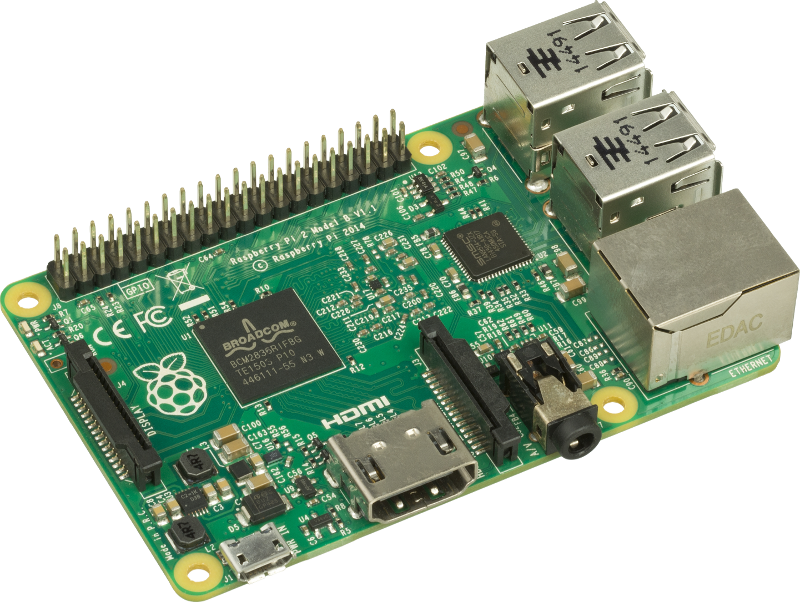
\includegraphics[width=0.56\textwidth]{res/raspberry}}
\caption{Raspberry Pi \cite{raspberry} with Broadcom System on Chip \label{fig:raspberry}}
\end{figure}
Actually almost all of the embedded systems use a SoC with similar boards, each one with its own size and configuration.

In order to accommodate many board implementations from different companies, each pin (or group of pins) of a SoC may have multiple configuration and operating modes.
The configuration of the pins is managed by the pin controller, a particular subsystem of a SoC.
Through a specific set of registers belonging to the pin controller, the system can configure the operating mode of the pins, such as their input or output mode.
These registers are typically accessible through a particular memory region called I/O memory. Such a kind of I/O access is known as \emph{Memory Mapped I/O}.

The features provided by a pin controller can be grouped into two main categories:
\begin{itemize}
	\item \itemname{pin configuration}: allows the system to change some electrical properties of the pins, such as direction, event detect, interrupt, etc.;
	\item \itemname{pin multiplexing}: each pin of the SoC may have many usages, also known as \emph{alternate functions}, depending on what is needed by the external board.
		The pin multiplexing feature enables the system to specify which type of function is needed on each pin.
\end{itemize}

As the I/O attack is a very low-level attack, it is necessary to dig further into the electrical world to know how these I/O interfaces work.


\subsection{SoC pins}
\label{sec:iopins}

I/O interfaces of a System on Chip provide a connection between internal modules and external electronic devices.
As shown in \myfig{fig:chips}, they are physically visible from the outside of the chip package,
usually in the form of pins \subref{fig:pins} or soldering balls \subref{fig:balls}.

\begin{figure}[h]
\centering

\begin{subfigure}{.45\textwidth}
\centering
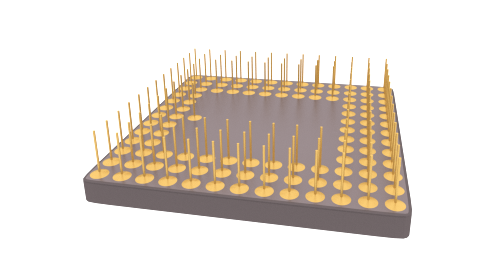
\includegraphics[width=\linewidth]{res/pins}
\caption{\label{fig:pins}}
\end{subfigure}
\begin{subfigure}{.45\textwidth}
\centering
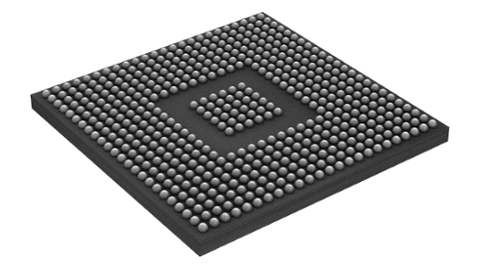
\includegraphics[width=\linewidth]{res/balls}
\caption{\label{fig:balls}}
\end{subfigure}

\caption{I/O connections packaged as \subref{fig:pins} Pin Grid Array and \subref{fig:balls} Ball Grid Array\label{fig:chips}}
\end{figure}

Internally they are connected to the silicon die through bonding wires, and are managed by a specific I/O circuit which may vary according to the specific chip.
Although there are many different implementations, almost all of the available SoCs have I/O ports with very similar functionalities.
For our purpose, we can describe them in an implementation-independent manner by using simplified generic schematics.


\subsubsection{Pin configuration}
\label{sec:pinconf}

The schematic depicted in \myfig{fig:pinconf} helps us to discuss about the first set of features: pin configuration.
The operation mode described in this section is also known as General Purpose I/O (GPIO).

\begin{figure}[h]
\centerline{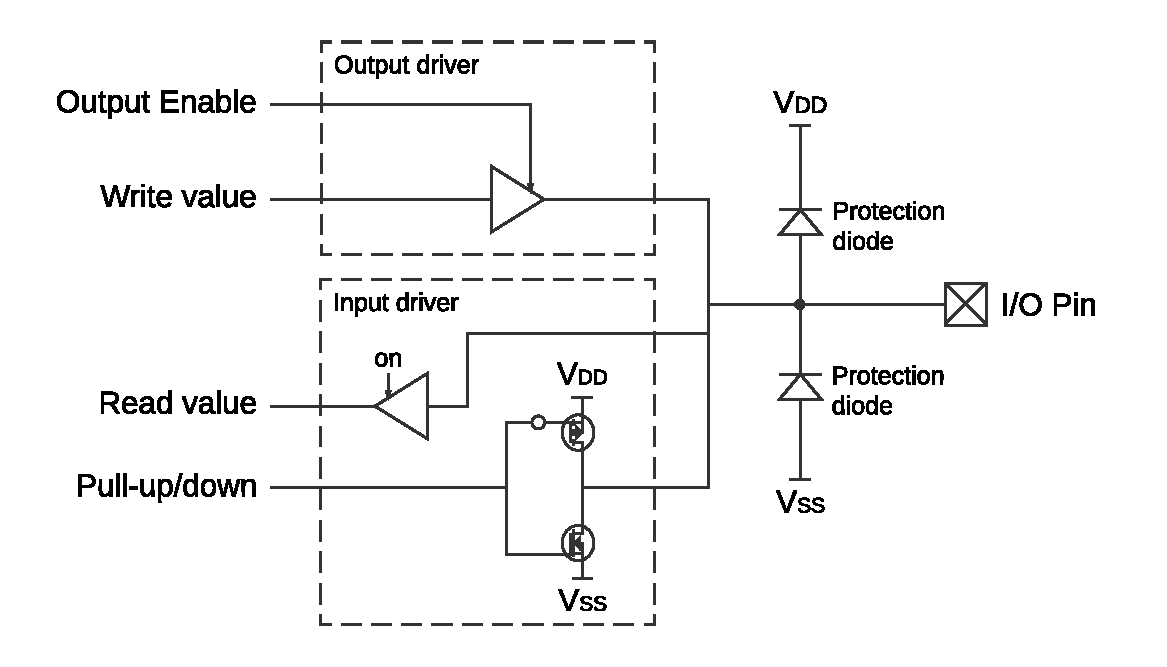
\includegraphics[width=0.8\textwidth]{res/pinconf}}
\caption{General Purpose I/O pin configuration circuit \label{fig:pinconf}}
\end{figure}

Apart from the protection diodes that serve as shield against input currents lower than $V_{SS}$ or higher than $V_{DD}$,
the circuit is divided into two different parts: one for output and one for input.
\begin{itemize}
	\item \itemname{Output driver}:
		The output module is basically a buffer controlled by an output enable signal.
		This signal controls the direction of the pin (input or output). If it is high, then the pin is in output mode
		and the value coming from a write operation goes through the buffer to the actual pin.
		If it is low, the pin is in input mode and the write signal is blocked, so it is not possible to change the external value of the pin from inside anymore.
	\item \itemname{Input driver}:
		The input driver has a similar buffer to read the value, usually having hysteresis capability which is useful for filtering unstable external values.
		Since the read buffer is always active, the input value is always available, even if the pin is currently working in output mode.
		The reason for this is merely physical: even if the external value was blocked by the buffer,
		one would always get a value by reading the input signal, because a value is nothing but an interpretation of the voltage level on a wire.
		When the pin is set as input, the pull-up/pull-down network enables the user to have a ``default'' value on the pin,
		namely a defined state maintained while the pin is not actively driven from outside. This feature is useful to avoid so called ``floating'' inputs.
\end{itemize}

For Pin Control Attack, what is more interesting about the circuit in \myfig{fig:pinconf} are the following two properties:
\begin{itemize}
	\item there is no checking about the input state, so it is possible to perform a read even when the pin is in output mode;
	\item vice versa, it is not possible to write to a pin which has been configured as output.
\end{itemize}

Furthermore, it is also possible to drive the pull-up/down network, factually disturbing the real value of the I/O pin in an unpredictable way.
Virtually, it is even possible to interfere with the pin value by means of external electromagnetic fields.
In these cases the effects strongly depends on the actual implementation of the printed circuit board as well as on the external components connected to the I/O pin.


\subsubsection{Pin multiplexing}

Inside the chip an I/O pin may be connected to more than one device, which can be selected depending on the application,
that is the way of soldering or wiring the package into an electronic board.
This SoC feature is known as pin multiplexing (also ball multiplexing, pad multiplexing, alternate functions).
Even though pin multiplexing is designed for hardware configuration, in almost all modern chips it is possible to change the function at run-time.

\begin{figure}[h]
\centerline{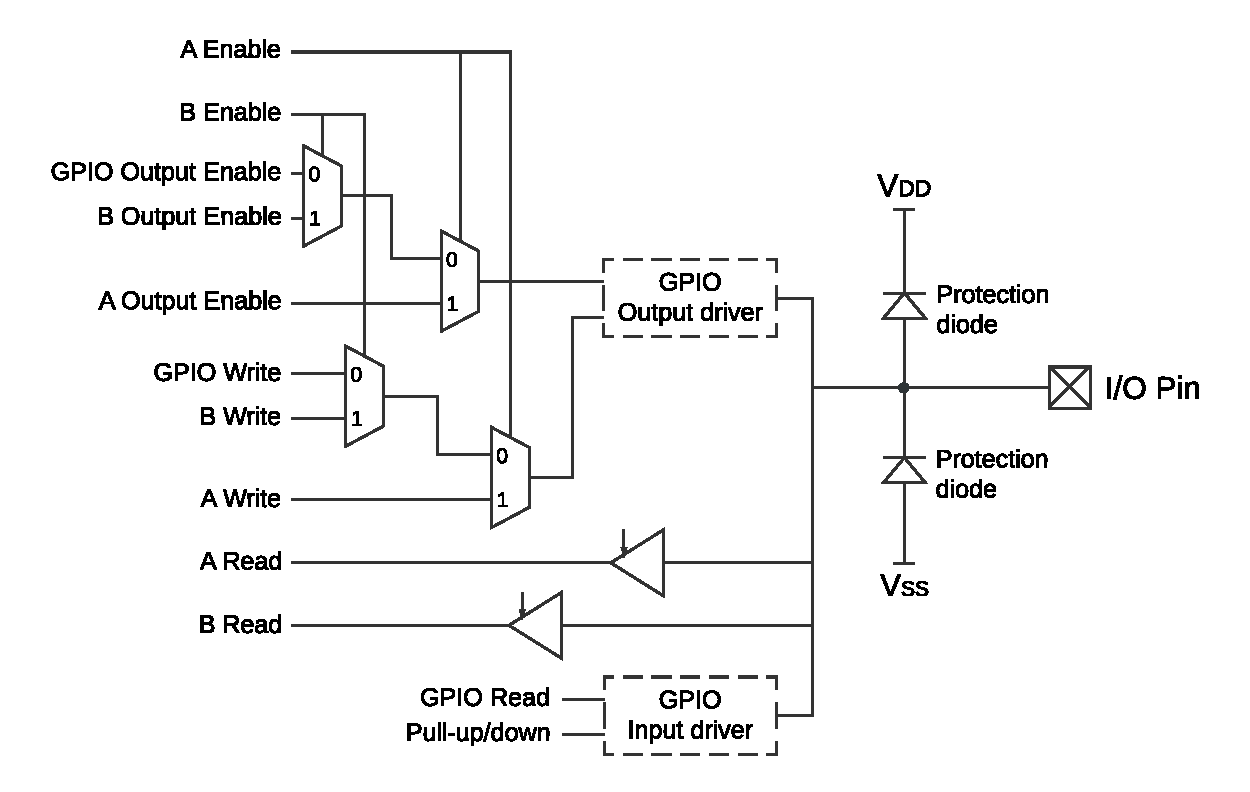
\includegraphics[width=0.8\textwidth]{res/pinmux}}
\caption{Generic I/O pin multiplexing circuit \label{fig:pinmux}}
\end{figure}

\myfig{fig:pinmux}~ shows a possible hardware implementation of pin multiplexing.
The I/O pin in the figure is connected to two different peripherals inside the chip, namely A and B,
and it is also accessible through basic GPIO as described in \mysec{sec:pinconf} above.
The access to the GPIO output driver is regulated by two in cascade multiplexers for each signal of the module.
If the peripheral A is enabled, then the signals driven by A go through the multiplexers and can drive the actual value of the pin,
while GPIO and peripheral B output signals are blocked. Instead, if only peripheral B is enabled then only its signals are able to reach the I/O pin.
Note that in this last case the peripheral A should not be enabled, because A multiplexers have precedence against B ones.
Thus, the cascading of multiplexers actually implements a priority mechanism between peripherals A and B.
If neither A nor B are enabled, then no alternate function is active for the I/O pin and it could be driven by GPIO signals.
Each peripheral may also have its own dedicated input line, to get values from the I/O port in the same way as GPIO does.

For our purpose, at least two interesting properties can be inferred from pin multiplexing schematic of \myfig{fig:pinmux}:
\begin{itemize}
	\item it is possible to block output signals from peripherals by simply changing the multiplexing configuration;
	\item the GPIO value can be read at any time, independently from the current multiplexing state of the output.
\end{itemize}


\subsection{PLC architecture}

As introduced in \mychap{chap:intro}, Programmable Logic Controllers are a particular kind of embedded systems,
designed to work into harsh environments and to control a physical process, typically an industrial or other critical processes.
In this section we examine the hardware and the software architecture of a PLC. This analysis will be needed later to better explain
the threat model and the implementation of Pin Control Attack.


\subsubsection{Hardware architecture}

Since it is built for working into a rough environment, the internal hardware of a PLC is shielded and not directly visible as the Raspberry Pi one.
\myfig{fig:wagoplc} shows an example of a basic PLC, provided by Wago. This model will be later used for our tests.
Note that, although we provide this specific example, the basic concepts described here are still valid for most of the PLC on the market, unless otherwise specified.

\begin{figure}[h]
\centerline{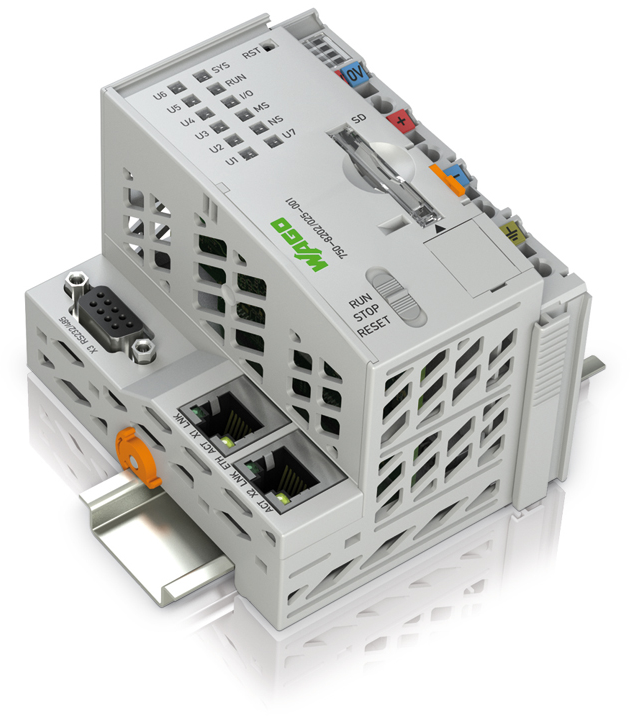
\includegraphics[width=0.5\textwidth]{res/wagoplc}}
\caption{PFC200 Programmable Logic Controller from Wago \label{fig:wagoplc}}
\end{figure}

Internally, the PLC has a System on Chip whose architecture is substantially equivalent to the one discussed in the above sections.
Therefore, the same concepts are applicable to PLCs as well.
Anyway, from our analysis we found that their architecture could be a bit more complicated with respect to a plain SoC.
Since the environment in which PLCs work may greatly differ case by case, they are designed to be as versatile as possible.
Vendors know that their PLC could be deployed in many different physical processes, possibly having completely diverse sensors and actuators to interact with.
Clearly, it is unreasonable to put every possible I/O interface on the same SoC. For this reason, most of the available PLCs comes with the possibility
of connecting a certain number of external components called \emph{I/O modules}. Each I/O module contains its own embedded SoC,
responsible for a specific subset of I/O interfaces (\eg digital input/output, analog input/output, pulse-width modulation, communication, etc.).
This hardware architecture is summarised in \myfig{fig:plc_arch}.

\begin{figure}[h]
\centerline{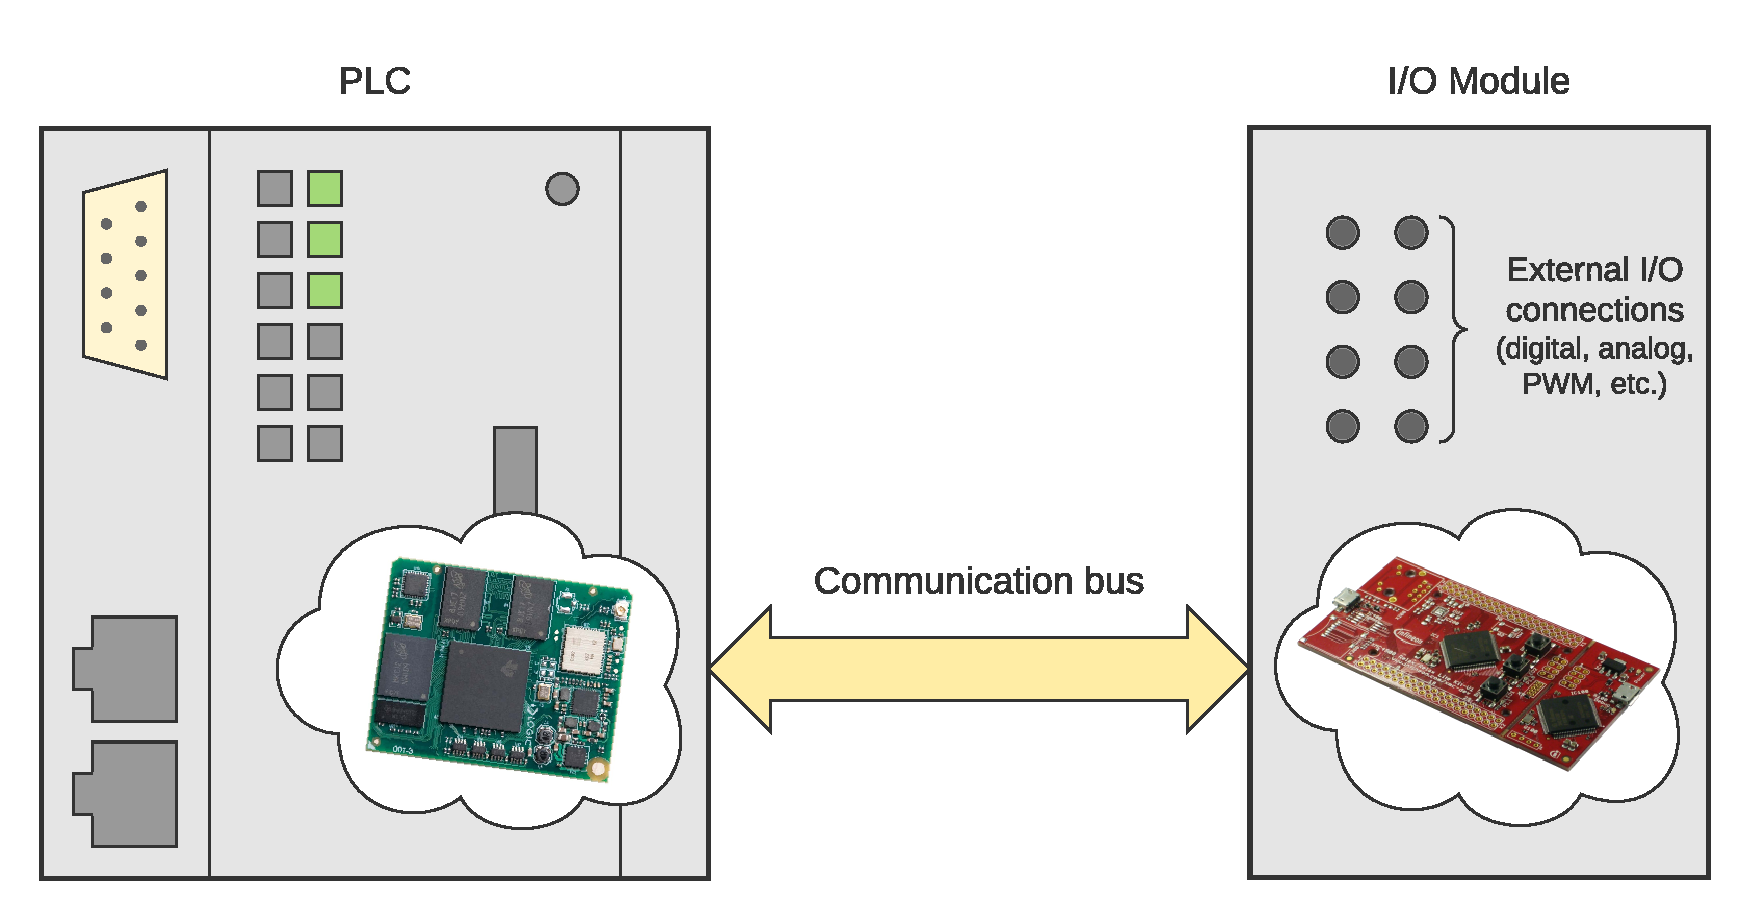
\includegraphics[width=0.8\textwidth]{res/plc_arch}}
\caption{PLC hardware architecture \label{fig:plc_arch}}
\end{figure}

The main portion of the PLC communicates with the I/O modules via a system bus, which is, in turn, connected to the I/O interfaces of the PLC.
This architecture with I/O modules adds one level of indirection between the targeted PLC and the external world, since there is another SoC in the middle.
Anyway, the same concepts of Pin Control Attack can be applied to such an architecture as well. It is sufficient to consider that the I/O interface of the PLC,
connected to the internal bus, is now the new direct target of our attack, while the final I/O becomes an indirect target. As we demonstrate in \mysec{sec:attack_plc},
by tampering with the I/O related to the communication bus it is possible to achieve equivalent results, proving that Pin Control Attack is still applicable on real PLCs.


\subsubsection{Software architecture}

The PLC typically comes with a real-time operating system (\eg Linux with RT-preempt patch, VxWorks etc.), because of the time requirements imposed by its main task.
Above the operating system, a software called \emph{PLC runtime} is responsible for managing the execution state of the control process and regulating the access to the PLC.
Through the runtime, the industrial operator can connect its terminal to the PLC and upload the desired control program, the \emph{logic}.
The PLC logic is the application code responsible for the control of the physical process, dealing with input and output interfaces.
As shown in \myfig{fig:plc_swarch}, this architecture can be divided into three layers, laying one above the other.

\begin{itemize}
	\item \itemname{Firmware}: the lowest layer, which basically corresponds to the operating system kernel. Although they are typically two distinct parts,
		here we consider the bootloader also as ``part'' of the firmware, because in this context their separation is irrelevant.
	\item \itemname{Runtime}: a software which is part of the application layer above the firmware, and it is started by the operating system itself.
	\item \itemname{Logic}: the control program running within the runtime environment. Its execution is started and stopped by the runtime,
		and its code is dynamic: it may change whenever the industrial operator decides to upload a new control program to the PLC.
\end{itemize}

\begin{figure}[h]
\centerline{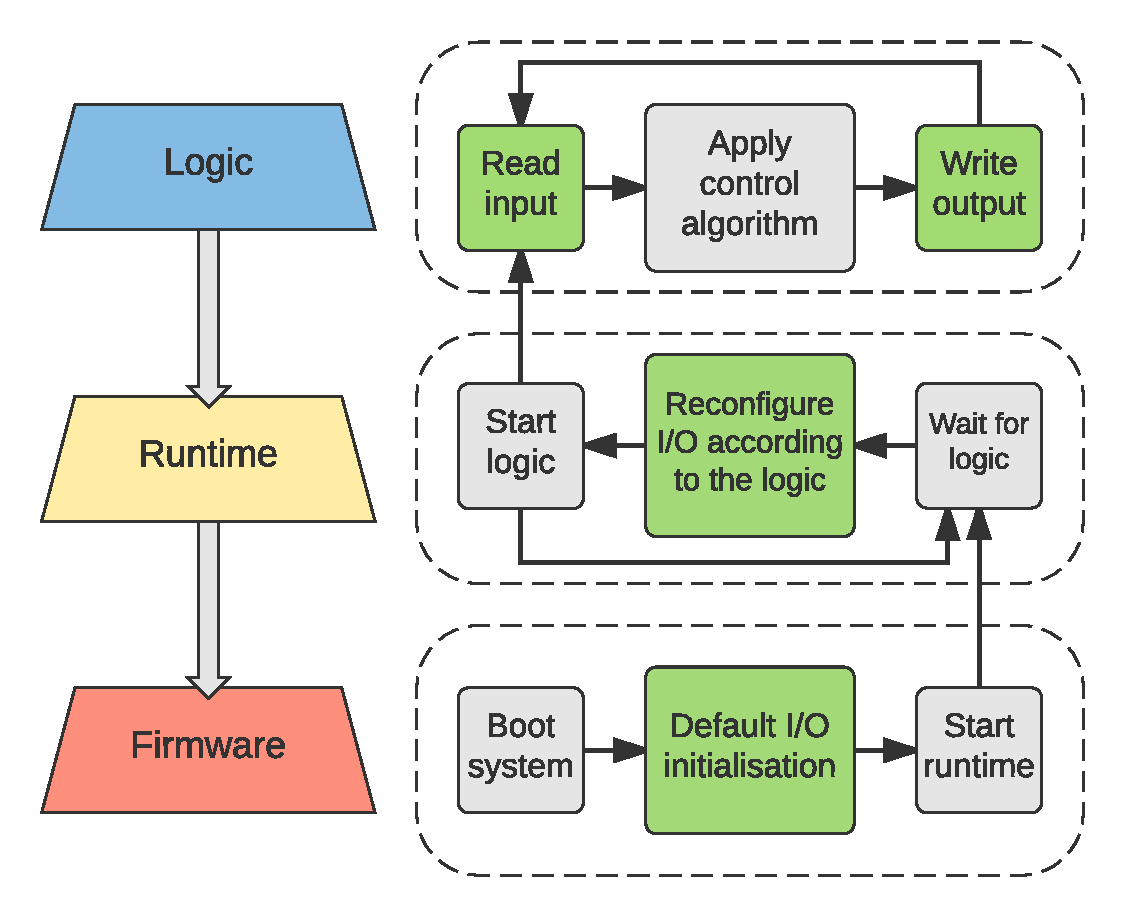
\includegraphics[width=0.7\textwidth]{res/plc_swarch}}
\caption{PLC software architecture \label{fig:plc_swarch}}
\end{figure}

\myfig{fig:plc_swarch} also summarises the execution flow of each layer, from bottom to top, highlighting (in green) the tasks directly related with the I/O.

When the firmware is loaded into memory and the system is booting, one of the early operation performed is known as I/O initialisation sequence.
In this phase, the drivers within the kernel configure their own I/O registers with their default values.
I/O initialisation includes both pin configuration and pin multiplexing. Normally, pin multiplexing is only performed at boot time, and, even though it is not forbidden,
pin multiplexing is never modified at run-time. Conversely, pin configuration may be changed later at run-time. Thus, depending on the implementation, the configuration
written during I/O initialisation may correspond or not to the one desired by the final application.

After the I/O has been initialised, the firmware loads the main application needed by the controller: the runtime.
The PLC runtime waits for a logic to be uploaded into the PLC from a terminal connected via the network interface.
The execution flow reported in \myfig{fig:plc_swarch} for the runtime layer is a general process, including the case when a PLC is started for the first time.
If a PLC is already in production, it is rarely restarted. However, when a reboot is needed (\eg for firmware update),
it may be configured to persistently save the current logic into a non-volatile memory and restore it after reboot.
In this case the ``Wait for logic'' step in \myfig{fig:plc_swarch} can be simply skipped, because a logic may be already available from disk.

When a logic is available, from network or from disk, the PLC runtime analyses its content.
The I/O configuration expected by a specific logic is bundled with the logic itself, because it is decided by the operator who has knowledge of the physical process
and knows how sensors and actuators are connected to the PLC I/O ports. With respect to the hardware architecture shown in \myfig{fig:plc_arch},
a change in the input/output required by the operator is actually reflected into a configuration change of the external I/O modules.
Whether this process involves a change in the I/O configuration of the PLC itself depends on the implementation and on the modification extend
(\eg if a new I/O module has been attached, this will probably require a change in the communication protocol and so on the I/O interface of the PLC).
After the new I/O configuration has been applied, the logic can be executed. From an operating system point of view, the logic is running in the same context of the PLC runtime.

As briefly discussed in \mychap{chap:intro}, the PLC logic executes the main \emph{scan cycle}. For each iteration, it reads from inputs, executes the control algorithm,
and writes to outputs. The control algorithm has been programmed by the industrial operator, and loaded through the interface provided by the PLC runtime.
When the logic is running, input and output pins have already been configured by the runtime, and the logic assumes that the I/O configuration does not change during its execution.
Both the logic and the runtime interacts with the I/O, but in different ways. The runtime deals with I/O configuration registers, while the logic performs read/write operations
related to I/O values. Both kind of interactions, anyway, require the same privileges, which will be later leveraged by Pin Control Attack.


\section{Attack Design}

Given the properties discussed in \mysec{sec:embed_arch}, it is possible to misuse the registers used to configure I/O peripherals,
and that is what Pin Control Attack does. This can happen at run-time, during the execution of the controller on a real process,
without any reaction from the PLC runtime or the operating system, thus remaining completely stealth.

We can argue that Pin Control Attack is actually applicable on any System on Chip having the
architecture described in \mysec{sec:embed_arch}. However, PLCs represent a particularly interesting target among all the embedded systems based on SoC.
PLCs leverage the interfaces of a SoC to interact with sensors and actuators, having direct effects on our physical world.
Therefore, if the I/O of a PLC is compromised, this constitutes a much more significant security and safety risk with respect to other
non-critical embedded system. For this reason, PLCs represent one of the most attractive targets for Pin Control Attack.

In this section we focus on the design of I/O attack. First, we summarise the host-based detection mechanisms taken into account
during the attack design and the techniques used to evade them. Second, we analyse the attack itself in more detail.
The goal of this chapter is to help us having a better understanding of the attack, and to provide a detailed threat model on which our defense design will be based on.

Pin Control Attack has been designed to be different from previous attack techniques, and to circumvent the off-the-shelf host-based detection systems.
The authors of I/O attack have identified two main defensive mechanisms whose properties makes them more easily applicable to PLCs.
Here we want to generalise and consider them in our threat model, clarifying how and when Pin Control Attack becomes applicable and interesting for attackers.
We also show how these defenses are circumvented by Pin Control Attack, and describe the available attack techniques.
We do not repeat here the detailed description made in \cite{ghostplc}. We only want to have basic concepts definition,
in order to be able to focus on our further analysis and implementation of the attack.


\subsection{Defense analysis}
\label{sec:def_analysis}

At this point, one could ask why descending to the lowest level possible to conduct an attack, when a lot of easier techniques (\eg function hooking) may achieve equivalent results.
The point here is that many producers of embedded systems and PLCs already started to move towards a more security-aware production.
As considered in \cite{ghostplc}, in order to be applicable to PLCs, a defensive mechanism should have at least the following properties:
\begin{itemize}
	\item low CPU overhead: CPU resources are limited in embedded systems such as PLCs, which typically have hard real-time constraints;
	\item designed to run on an operating system: almost all of the modern PLCs have a real-time OS running on it;
	\item no hardware modification required: many solutions are hardware-based \cite{trustlite,hardware-ibmac,ocfmm,fine-grained,bb-cfi}, making them not easily applicable;
	\item no virtualisation required: the majority of embedded systems, like PLCs, does not support virtualisation;
		thus solutions like \cite{hypervisor-control} are less attractive.
\end{itemize}

Given these considerations, we can list some of the applicable defenses:
\begin{itemize}
	\item \itemname{SEM}: the Symbiote detection system described in \cite{symbiotes}, which protects the kernel from code modification attacks;
	\item \itemname{Autoscopy Jr.}: the lightweight intrusion detection system proposed in \cite{autoscopy}, effective against control flow manipulation inside the kernel.
\end{itemize}

The above detection systems still have some shortcomings, leveraged by Pin Control Attack.
First, they are based on a comparison with golden references (the symbiotes and the TLL, respectively) taken from a subset of the entire kernel space.
If the attacker is able to find a portion of the kernel space which has not been considered by the detection system, then it can be circumvented.
For example, Autoscopy Jr. can be bypassed if the attacker is able to craft a duplicate of the kernel functions it needs.
If a duplicate function is used instead of the original version, Autoscopy Jr. does not throw an alert, because this function is not listed in the TLL at all.
Second, the references used by both defenses are \emph{static}, which means that they are based on previous analysis of the immutable (static) portion of the system.
Thus, an attacker could still use dynamic memory, whose content changes during run-time, to conduct its own attack.
In the case of SEM, only static code regions (which are immutable) are taken into account, so any malware placed in dynamic memory will not be detected.
Autoscopy Jr., instead, considers the function pointers used inside the kernel, including the ones inside the System Call Table and other similar tables.
Therefore, it is able to detect only \emph{data hooks} but not \emph{code hooks}, that is, any direct code modification (\eg of the kernel text) is still possible.

Anyway, these two defenses may be used in combination, thus providing a host-based IDS able to detect both code and data hooks.
Even if they are deployed together, however, attacks through dynamic memory and without function hooking are still possible,
since monitoring dynamic memory is a far more complex issue. One of the implementations of Pin Control Attack (see \mysec{sec:attack_impl})
leverages exactly the kernel dynamic memory to reach its purpose.

Host-based detection mechanisms like the ones discussed above will likely be deployed into many commercial products within the next years \cite{symbiote_web, autoscopy_web},
raising the bar for attackers. Therefore, Pin Control Attack will become more and more interesting as long as classical techniques (\eg function hooking) are overcome.


\subsection{Threat model}
\label{sec:threat_model}

In our work, we assume that the system is protected at least by the HIDSs described in \mysec{sec:def_analysis}, or equivalent.
Hence, we assume that the attacker cannot tamper with operating system (kernel) functions and data structures, but it can still use dynamic memory to insert its malicious code
and tamper with the I/O configuration. The attacker can also write its own version of kernel functions if needed, and call them separately in order to avoid HIDSs.
This approach, anyway, requires very high effort and would really be the last option for an attacker.

The attacker, depending on the attack implementation, may need different running privileges on the target system to execute Pin Control Attack.
Generally speaking, the minimum privilege required is the privilege level of the PLC runtime, which has access to the I/O configuration registers.
As already discussed in \cite{ghostplc}, many ICS-CERT advisories have shown that PLCs have vulnerabilities that could lead to malicious code execution
\cite{plc-network,abb-codesys,codesys-server,schneider-bof,rockwell-vuln,rockwell-vuln2}, and they may affect PLC runtime software as well.
Thus, obtaining the same PLC runtime privilege level is feasible on real systems.

As in \cite{ghostplc}, we assume that the attacker knows both the physical process controlled by the target system and the mapping
between I/O configuration and external sensors and actuators. The former is typically known by the attacker, which has reasonably studied its target before conducting the attack.
This is confirmed by Stuxnet \cite{stuxnet}, where attackers had very deep knowledge of target system and physical process.
The latter is given by a knowledge of the PLC logic, which, as said, already comes with the mapping between I/O interfaces and control variables used by the logic.
Furthermore, the research presented in \cite{dynamic-payload,sabot} shows that it is possible to infer the structure of the devices connected to the PLC and used by the logic,
factually lowering the bar for attackers which do not need an a priori knowledge of the I/O mapping anymore.


\subsection{Pin Control Attack}

Based on the previous assumptions, Abbasi et al. \cite{ghostplc} crafted Pin Control Attack, which is capable of manipulating the physical process
controlled by a PLC without requiring any firmware or logic modification.
The idea of Pin Control Attack is that the attacker operates at the lowest level possible, targeting the interaction
between the firmware and the I/O, as shown in \myfig{fig:target}. For this reason the attack is also known as I/O attack.
Despite its crucial function in embedded systems, I/O hardware architecture and I/O drivers are currently designed
without taking into account any concept of security, assuming that I/O is reliable. Unfortunately, given the properties inferred in \mysec{sec:embed_arch}
from a generic hardware architecture, this is often not the case.

\begin{figure}[h]
\centerline{\includegraphics[page=6,viewport=50 620 300 750,clip]{res/ghostplc}}
\caption{Pin Control Attack target, from \cite{ghostplc} \label{fig:target}}
\end{figure}

As described in \cite{ghostplc}, Pin Control Attack is designed to evade off-the-shelf HIDSs presented in \mysec{sec:def_analysis}.
In particular, it leverages kernel dynamic memory (in one implementation variant) or it uses a simple user code (in a second variant).
Both variants are able to circumvent the above detection mechanisms.

The authors of \cite{ghostplc} have found at least two different attack vectors for Pin Control Attack: \emph{Pin Configuration} and \emph{Pin Multiplexing}.
Both kind of attacks leverage the SoC properties described in \mysec{sec:embed_arch}.
The attack is performed by misusing the control registers used to program the I/O peripherals, writing malicious values into them.
If the attack targets I/O configuration registers, it is a Pin Configuration Attack, otherwise, if the targeted registers are related to the multiplexing state of the pins,
then it is a Pin Multiplexing attack. In some architectures, I/O configuration and multiplexing is achieved by using the same set of registers
(\eg different bits of the same register may have different purposes).

In both cases, the main principle behind the attack is something that they called \emph{memory illusion}, which is represented in \myfig{fig:illusion}.
In a system equipped with a Memory Management Unit (MMU), that is the most common scenario for PLCs, each process cannot directly access to physical address space.
Every memory access is mediated by the MMU, which creates an abstraction called \emph{virtual address space}, or \emph{virtual memory}.
When a process wants to access physical memory, it has to request a mapping to the system between physical address space and virtual address space.
In this way, every process has its own ``virtual view'' of the physical memory. This is valid also for I/O memory, which is part of the physical memory.
Once a mapping has been established, the I/O can be managed by accessing the mapped virtual memory.
\begin{figure}[h]
\centerline{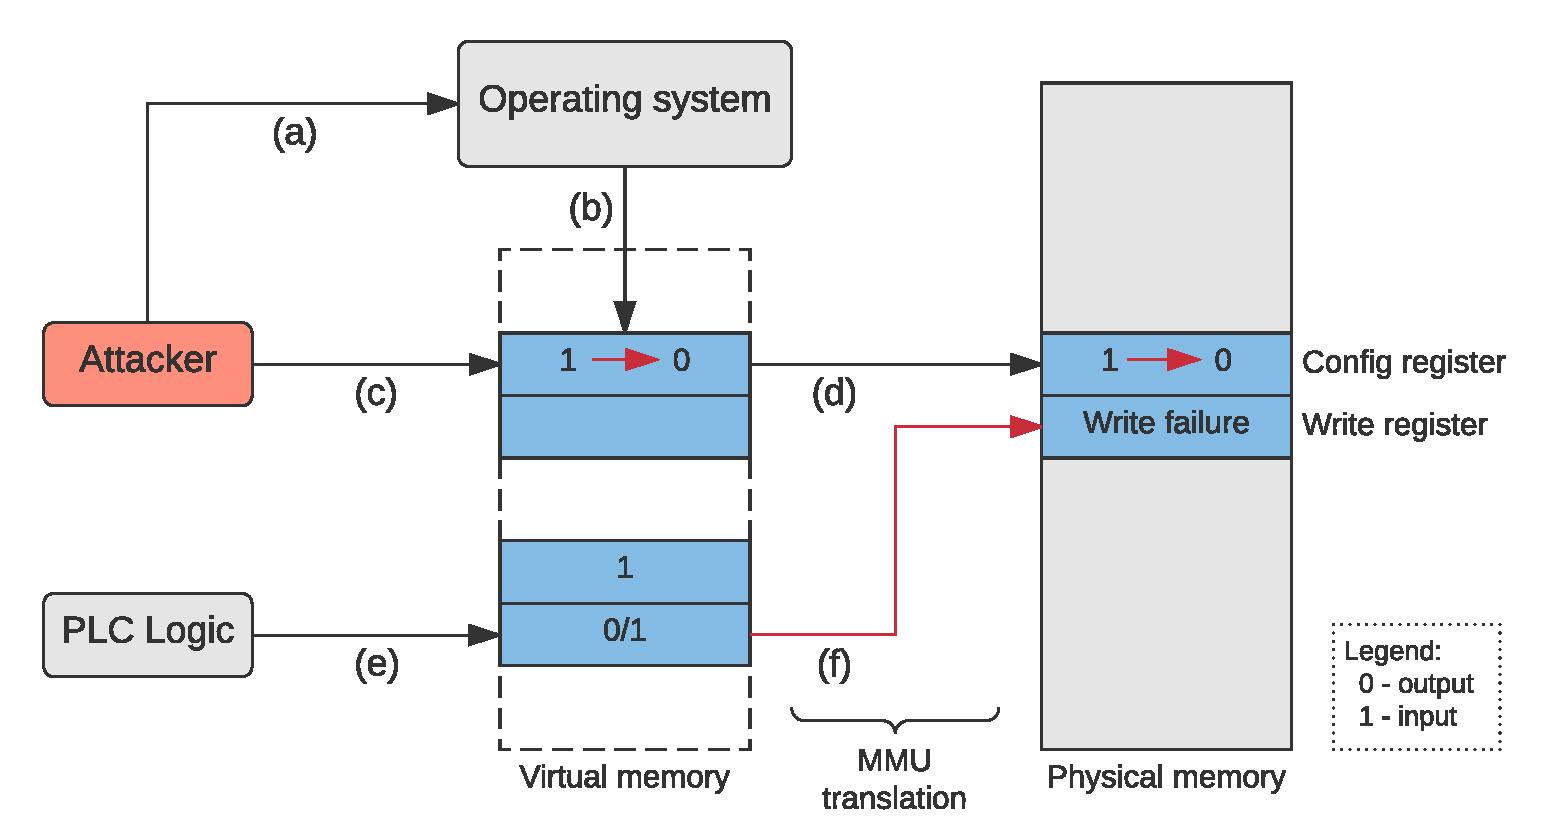
\includegraphics[width=0.9\textwidth]{res/illusion}}
\caption{Pin Control Attack memory illusion \label{fig:illusion}}
\begin{minipage}{0.1\textwidth}
\phantomsubcaption{\label{fig:mapping_request}}
\end{minipage}
\begin{minipage}{0.1\textwidth}
\phantomsubcaption{\label{fig:mapping_provided}}
\end{minipage}
\begin{minipage}{0.1\textwidth}
\phantomsubcaption{\label{fig:conf_change}}
\end{minipage}
\begin{minipage}{0.1\textwidth}
\phantomsubcaption{\label{fig:phys_change}}
\end{minipage}
\begin{minipage}{0.1\textwidth}
\phantomsubcaption{\label{fig:virt_write}}
\end{minipage}
\begin{minipage}{0.1\textwidth}
\phantomsubcaption{\label{fig:write_failure}}
\end{minipage}
\end{figure}
Thus, as \myfig{fig:illusion} outlines, an attacker can do the following: first, it has to request a mapping for I/O memory \subref{fig:mapping_request};
once a virtual mapping is provided by the operating system \subref{fig:mapping_provided}, the malicious process is able to alter the pin configuration (\eg change an output pin to input)
through virtual memory \subref{fig:conf_change}. This change is immediately reflected into physical memory via MMU translation \subref{fig:phys_change}. When the PLC logic,
which is a normal process in the system, tries to update the value of the pin through virtual memory \subref{fig:virt_write},
the target address of the write instruction arrives to the MMU, which translates it to the corresponding physical address.
Unfortunately, since the pin has been changed to input, the execution of the instruction does not actually affect physical memory \subref{fig:write_failure}.
Therefore, the write silently fails, but no signal error is reported back to the CPU, and from the process virtual perspective everything went correctly.
As explained later in \mychap{chap:defense}, the fact that the virtual address of the instruction actually reaches the MMU will be a crucial mechanism
for the design of our defense.

As reported in \cite{ghostplc}, only by leveraging the configuration of pins they crafted an attack which is able to do the following:
\begin{itemize}
	\item reconfigure an I/O pin as input when the PLC logic is attempting to write;
	\item reconfigure an I/O pin as output and write a malicious value when the PLC logic is attempting to read.
\end{itemize}
In this way, the attacker can make specific write operations fail and can feed the PLC logic with malicious input values at the same time.
We discuss about some limitations of this approach in \mysec{sec:attack_impl}.

Moreover, we imagine that many other attack possibilities may exist. An attacker can tamper with the I/O configuration in many other ways depending on the
specific I/O peripheral and on its features (\eg event detect, interrupts, clock signals, etc.), and the effects of the attack are unpredictable.
If the attacker can analyse the reference manual of the target SoC (mostly publicly available) and it has enough competence and time,
the only limit to Pin Control Attack becomes fantasy.
To give an idea of what such an attack can do, imagine a simple SoC pin which can be multiplexed between a memory controller and a PWM controller.
If this pin is actually connected to an external memory, thus multiplexed as memory controller, a Pin Multiplexing attack can lead to dangerous signals
sent from a PWM controller to a memory module, which may burn the memory.

On the other side, from our analysis on a real PLC, we found that another attack vector is viable at a different abstraction level than hardware configuration.
Commonly, the I/O peripherals are used through operating system drivers, which in turn are used from user space applications like the PLC runtime.
As we show in \mysec{sec:attack_plc}, an attacker can target these drivers, or even these applications, to obtain equivalent effects without dealing with
the underlying hardware and/or I/O registers directly.


\section{Attack Implementation}
\label{sec:attack_impl}

In this section we first describe the available implementation presented in \cite{ghostplc}, which was the starting point of our analysis.
Next, we introduce a possible attack implementation on a real PLC. Both implementations are designed for Linux systems, and they have two different
variants: kernel side and user side. Each variant imposes different requirements for the attacker, which will be discussed in more detail in the next sections.


\subsection{Raspberry Pi}
The system used for our experiments with the first implementation is a \emph{Raspberry Pi 1 Model B} based on an ARMv6 architecture, running the following kernel:
\begin{Verbatim}[fontsize=\small]
	Linux raspberrypi 4.4.22+ #912 Mon Sep 26 19:00:13 BST 2016 armv6l GNU/Linux
\end{Verbatim}
The Raspberry Pi 1 features a Broadcom System on Chip named \emph{BCM2835}. With reference to the BCM2835 documentation \cite{bcm2835},
we set up the system I/O by connecting a button as input, an LED and a servo motor as outputs. Button and LED are accessed via $2$ GPIO interfaces,
one configured as input and one as output, respectively. To connect the micro servo, we needed an external PWM controller. The controller is attached to the system
through the I2C interface, which requires two pins: one for the data line, \emph{Signal DAta} line (SDA), and one for the clock line, \emph{Signal CLock} line (SCL).
The resulting system on which we conducted our experiments is shown in \myfig{fig:pi_system}, and its I/O configuration is summarised in \mytab{tab:pi_pins}.

\begin{figure}[h]
\centerline{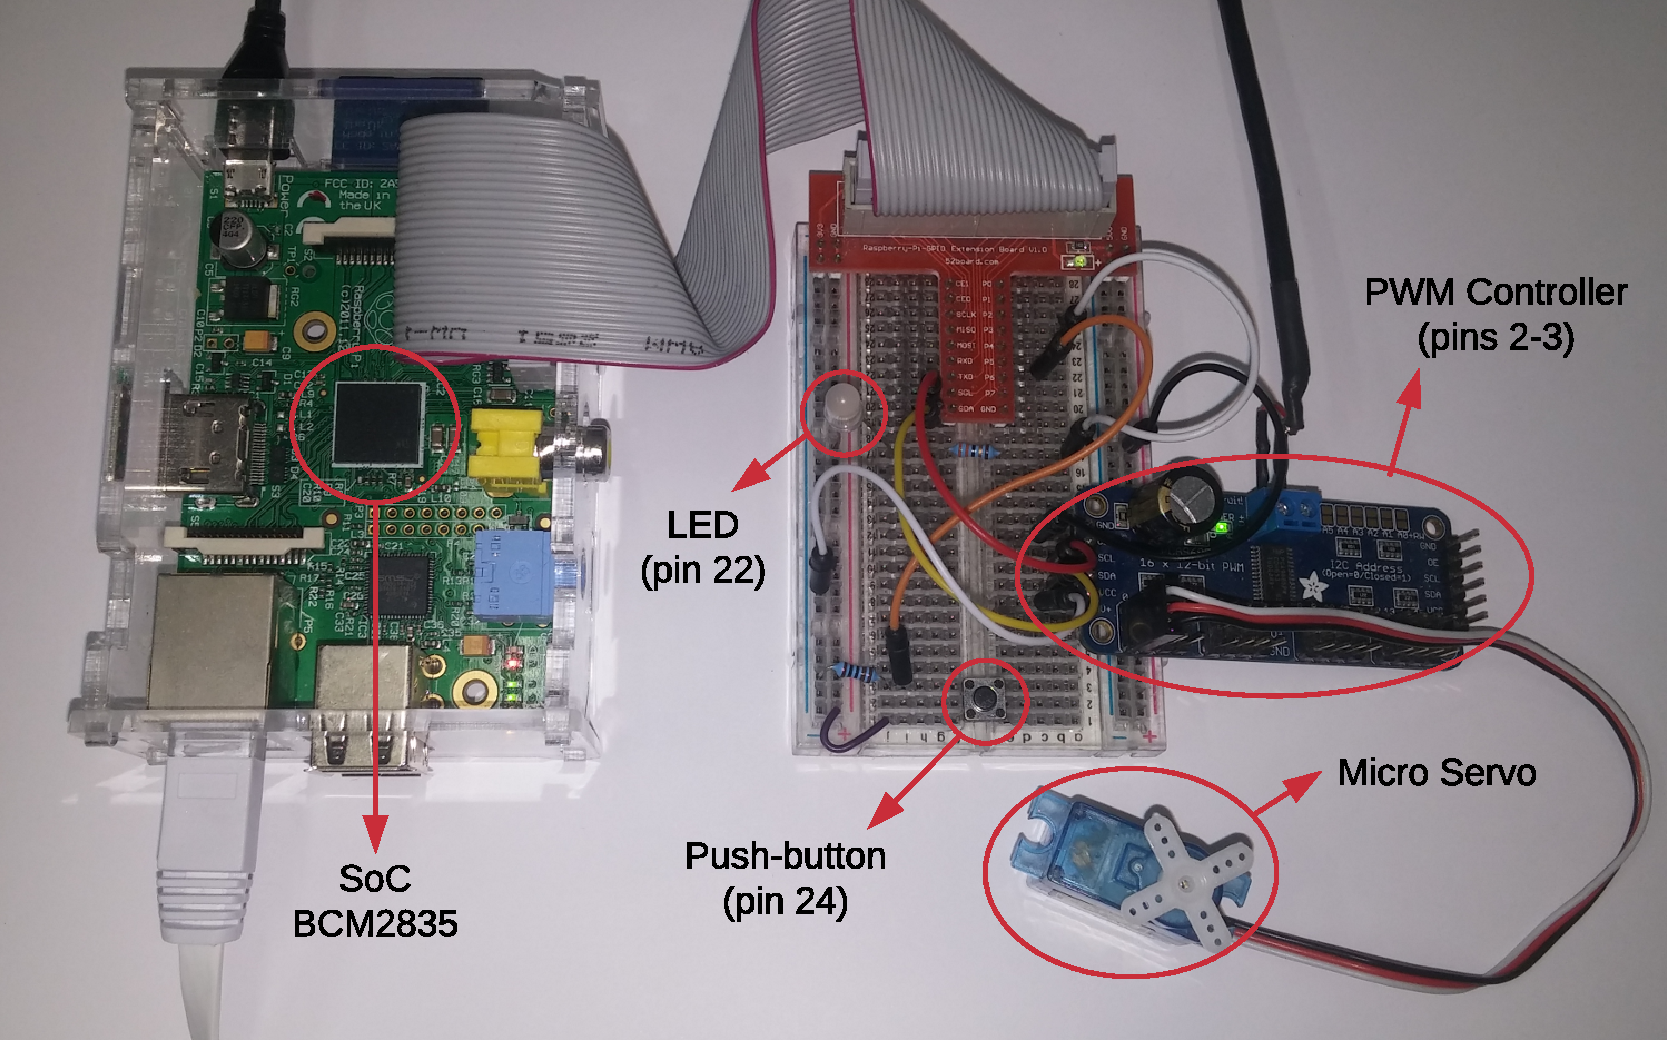
\includegraphics[width=0.8\textwidth]{res/pi_system}}
\caption{Raspberry Pi system used for experiments \label{fig:pi_system}}
\end{figure}

\begin{table}[h]
\centering
\renewcommand{\arraystretch}{1.5}
\begin{tabular}{|c|c|c|c|}
\hline
\thead{Pin} & \thead{Multiplexing} & \thead{Configuration} & \thead{Connected to} \\
\hline
24 & GPIO & Input & Button \\
\hline
22 & GPIO & Output & LED \\
\hline
2 & I2C SDA & - & PWM controller (servo) \\
\hline
3 & I2C SCL & - & PWM controller (servo) \\
\hline
\end{tabular}
\caption{I/O configuration of our Raspberry Pi testing system}
\label{tab:pi_pins}
\end{table}

To enable PLC capabilities on such a system, we installed a PLC runtime on it. In particular, we used \emph{CODESYS Control for Raspberry Pi SL}
provided by 3S-Smart Software Solutions GmbH \cite{codesys_runtime}. Through the CODESYS Development System \cite{codesys_dev},
we designed the PLC logic shown in \myfig{fig:pi_logic}, whose code is executed for each scan cycle.
\begin{figure}[h]
\centerline{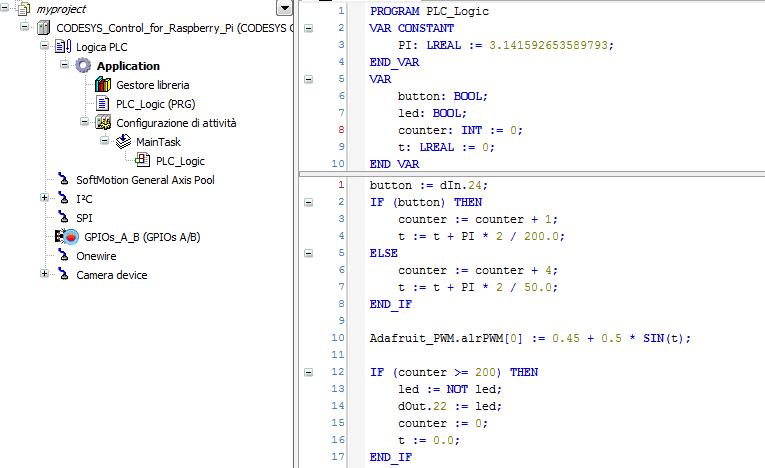
\includegraphics[width=0.8\textwidth]{res/pi_logic}}
\caption{PLC logic loaded into the target system \label{fig:pi_logic}}
\end{figure}
We chose a $10ms$ scan cycle interval, however, since this PLC runtime is not real-time, the timing may be affected by small errors ($\approx 50\micro s$).
At each scan cycle, the logic reads from pin 24 (push-button), and writes the outputs accordingly.
The motor is driven with a sinus wave which makes it going forward and backward in the interval $[-45^\circ, +45^\circ]$.
If the button is not pressed, which corresponds to value $1$ (high), the LED is toggled every $2s$ and the motor completes a round in $2s$.
If the button is pressed, that is value $0$ (low), both LED and motor frequencies are multiplied by $4$, and the new round time becomes $500ms$.
The timing of the write operations, which is a multiple of the scan cycles, is controlled by software counters embedded into the logic.
Thus, while the input is high the counters are updated at normal speed; while the input is low they get updated $4$ times faster.

Given the system above, a possible implementation of Pin Control Attack can target input or output pins, having different effects.
By reconfiguring an output pin as input, it is possible to disable the PLC logic write operations.
Instead, by changing an input pin into output, and writing its own values, an attacker can actually modify the behaviour of the outputs.
In our case, if the attacker is able to intercept PLC logic read operations and write its own values, he can actually decide the frequency of the outputs.
For instance, as demonstrated by our attack experiments, if the attacker feeds the logic with $0$ and $1$ alternatively at each scan cycle,
the round time of the outputs becomes the average between $2s$ and $500ms$, factually having a frequency that is not even programmed into the logic.
But there is a limitation to this attack approach, implied by the architecture described in \mysec{sec:pinconf} and confirmed by the experiments:
the read operation is not reliable if the pin is configured as output pin. In our case, if we reconfigure pin 24 as output, the malicious value written into the write register
is not always the same value read by the PLC logic. That is probably because the voltage on the pin is actually driven by two entities at the same time,
the external sensor (the button) and our attack, so it is not deterministic whether, at the time of reading the pin level register, the voltage is considered a $1$ or a $0$.

The authors of Pin Control Attack described two different ways of intercepting read (or write) operations, and they implemented them into the following attack variants:
\begin{enumerate}
	\item a Linux loadable kernel module which is able to intercept logic read and write operations by leveraging the \emph{Debug subsystem};
	\item a user code which maps the physical I/O memory, or re-use PLC logic mapping, and manually watches the I/O values to synchronize itself with the PLC logic operations.
\end{enumerate}
Once the target operation has been caught, the attack modifies the I/O configuration according to its purpose.
Both implementations are able to evade the HIDSs analysed in \mysec{sec:def_analysis}, because they reside into kernel and user dynamic memory, respectively,
and they do not alter any control flow. Here follows a brief description of these two possible implementations, focused on the findings of our experiments.
For a more detailed analysis of the original version of the attacks refer to \cite{ghostplc}.


\subsubsection{Kernel module}
This variant requires root privileges, in order to be able to insert a loadable module into the kernel.
The kernel module makes use of debug registers, available in many embedded architectures, to catch PLC logic operations.
A debug register takes a virtual address, and optionally a process context, and raises a CPU exception when the address is accessed within the given context.
The access type may be read, write or execute: the first two are intended for data addresses, the last one for instruction addresses.
Thus, to use a debug register, the attacker needs to know the mapped virtual address used by the PLC logic to read/write the I/O pins.
These addresses are typically mapped by the PLC runtime before starting the logic, and can be easily obtained by looking into the \verb|/proc/<pid>/maps|
file, which lists the current mappings owned by a process identified by \verb|pid| (process id).
As discussed in \mysec{sec:threat_model} the attacker needs to know the running PLC logic, and so the mapping between the I/O pins and
the physical process he wants to tamper. With reference to our target system, if the attacker knows that the input button is connected to pin $24$
and wants to intercept a read operation, then he can get the physical address of the read register from the SoC documentation \cite{bcm2835} (\verb|0x20200034|),
and finally the virtual address from the current PLC runtime mappings (\eg \verb|0xb6f40034|). With this information, he can install a debug exception handler
by setting a debug register: the malicious handler will be called whenever the PLC logic tries to read from that address.
Inside the handler, the attacker can decide whether to change the pin configuration and which value wants to feed the PLC logic with.
The use of debug registers gives the attacker a great timing accuracy on read and write operations,
but the overhead may be detectable by power consumption-based intrusion detection systems.


\subsubsection{User code}

This version does not need root privileges as the previous one. Since it is executed from user space, to have access to the I/O physical memory it needs to either
request a new mapping to the kernel or use the existing mapping of the PLC runtime. In both cases, the requirement is to have the same privilege level of the PLC runtime,
and this may be obtained by exploiting a code execution vulnerability affecting the Codesys PLC runtime \cite{abb-codesys,codesys-server}.
The requirement needed to obtain the PLC runtime mapping is the same as the kernel module variant.
To intercept read and write operations, the attacker cannot use debug registers, because the access to the debug subsystem is mediated by the kernel \verb|ptrace| API.
Therefore, this version can only monitor the value of an output pin to get the relative time, and also infer timing information of other pins
by using its knowledge of the PLC logic. In our case, if the attacker monitors the pin $22$, when its value changes he knows from the logic
that at the same time the button input has been read, and the servo motor has just finished a round.
This information can be used to set relative timers, which will be activated on the next I/O events.
If the target system has real-time capabilities, as almost all real PLCs do, this technique can be even more accurate than our experiments in a non real-time environment.
Moreover, its overhead is much less than the corresponding debug register one, and it may not be easily detectable.


\subsection{PLC}
\label{sec:attack_plc}

TODO PLC implementation.


\chapter{Attack detection}
\label{chap:defense}

This chapter proposes a possible countermeasure to I/O level attacks.
First, it describes the overall design of our detection system, showing the approaches to tackle the attack at different levels
and explaining our design choices. Second, it contains a detailed report of the implementation for Linux kernel.


\section{Design}
We report the design phase below, starting from a preliminary analysis of the problem to a discussion of different possible solutions.
Then, a detailed description of the defense architecture concludes the section.


\subsection{Preliminary analysis}
\label{sec:pre-analysis}

The main goal of our defense is to detect and hinder I/O attacks while being able to not consume the limited resources inside the target system,
and to not affect real-time operations. The timing of the operations is fundamental in systems like PLCs, on which the minimum delay may alter the physical process.

We make the same assumptions contained in the threat model of \mysec{sec:threat-model}.
Therefore, we assume that the system, and our defense as well, is protected by the previously discussed HIDSs.
Starting from the analysis reported in \mychap{chap:attack}, we identify the I/O configuration as the main resource we aim to protect.
To target I/O configuration, the attacker may use other system capabilities, such as virtual address mapping and debug registers.
First of all, we define the following components of a SoC, to which we refer several times in the rest of the paper:
\begin{itemize}
	\item \itemname{I/O subsystem}: the subsystem that controls the I/O configuration. I/O configuration is defined as the set of all the control registers
		actively used by the SoC, whose unauthorised modification may have direct or indirect effects on the controlled process.
		In particular, we are interested into pin control registers, which directly determine the behaviour of the SoC I/O pins.
		However, a SoC typically contains many devices and controllers which may be in charge of a subset of I/O pins. In other words, some pins
		can be multiplexed to specific devices inside the SoC. Since these devices are programmed through their own control registers,
		altering these registers may indirectly affect I/O pins as well. Thus, both pin control registers and device control registers
		are considered as part of the I/O configuration. The attacker who has knowledge of the system and its I/O peripherals may access
		all these registers to alter the physical process.
	\item \itemname{Debug subsystem}: the SoC subsystem that enables debug capabilities for the operating system and its processes.
		Typically, it consists of a set of registers, called \emph{debug registers}, inside the processor of the SoC.
		The operating system may provide an interface to access them, both for kernel side and user side.
		The attacker may leverage the debug subsystem to obtain accurate timing information and conduct more sophisticated attacks,
		either using the interface provided by the operating system or the low-level processor instructions directly (depending on its privilege level).
	\item \itemname{Mapping subsystem}: the system that manages mappings between physical and virtual addresses, both for kernel and user space.
		It is typically supported by the Memory Management Unit (MMU) in hardware, and by the operating system in software. Within the context of a PLC,
		the runtime may use this subsystem to configure the I/O and to perform read/write operations. An attacker can access physical I/O addresses
		(thus, I/O configuration) either by requesting a new mapping to the system or by using an already existing mapping.
\end{itemize}

Given the architecture described in \mysec{sec:embed-arch}, protecting I/O configuration is not straightforward because the hardware lacks
any protection mechanism related to the I/O subsystem. For instance, the SoC might generate a trap for each modification to I/O registers.
However, this approach would not be reasonable, because of the huge overhead imposed to any I/O access.
Alternatively, a trap could be generated only when an I/O access is malicious. For example, to prevent pin configuration attack,
a trap signal might be delivered to the CPU when the internal signal of a pin is different from the external one, meaning that the pin is misconfigured.
A similar approach may be used for pin multiplexing, by checking the internal signal connected to the multiplexed device.
Unfortunately, since these approaches would require significant hardware modifications, with subsequent updates of all the SoC drivers, they are very unlikely to be applied.

Thus, we need to define an alternative approach that does not have the above limitations: it must be easily applicable and have a minimal overhead.
Since the hardware-based solution is unpractical, we analysed the possible software-based solutions.
In order to choose the best strategy against Pin Control Attack, we compared the following approaches, as proposed in \cite{ghostplc}:
\begin{enumerate}
	\item monitoring I/O configuration to detect changes;
	\item monitoring the use of debug registers;
	\item monitoring the mapping requests targeting I/O configuration;
	\item monitoring performance overhead;
	\item using a trusted execution environment.
\end{enumerate}
These approaches are not mutually exclusive, and may be used simultaneously to get a higher protection level.
In this work, we decided to design and implement the first three approaches in combination, because they directly protect the three different resources that the attacker may use.
Thus, they represent a good minimum set of countermeasures capable of raising the bar for the attacker (see \mysec{sec:def-arch}).
Our solution, however, may be extended to include the last two approaches as well, to cover some existing limitations (see \mysec{sec:def-sec}).
Before describing our design phase, we briefly discuss these two further protections in the following sections.


\subsubsection{Monitoring performance overhead}

A detection system based on performance monitoring may be useful to add a further protection, especially against the attack variant
which uses debug registers. In general, such a monitor would be also useful for other kind of attacks targeting PLCs, because these systems cyclically performs
a limited amount of well-known operations. This simplifies the detection of any deviation from the standard behaviour.
In our case, a performance monitor would be helpful to cover those attacks that the first three strategies are not able to detect,
although, as discussed in the following sections, those are very limited cases.
Deploying a performance monitoring system, anyway, does not require very high effort because it can leverage \emph{Hardware Performance Counters} (HPC),
nowadays available in almost all the SoC processors. The most challenging part would be, of course, integrating the monitor with the PLC runtime.
When a new logic is uploaded to the PLC, a burst of operations are executed by the runtime to check the new logic code, apply the new configuration and start the logic.
These extra operations, of course, must not be labeled as malicious. Furthermore, once a new logic started, it may perform operations that are different
with respect to the previous one; therefore, the monitor should be able to recognise this change and update its statistics as well.


\subsubsection{Trusted execution environment}

A Trusted Execution Environment (TEE) is a particular set of hardware and software components providing security features,
such as isolated execution, integrity of Trusted Applications (TAs), and integrity and confidentiality of TAs assets \cite{tee}.
The TEE technology is based on the concept of partitioning a computing system into Secure and non-Secure world, where
the code running into non-Secure world cannot access the Secure partition.
A lot of effort has been put into the standardisation of the TEE, and some commercial solutions already exist,
such as Intel Trusted Execution Technology (TXT) \cite{intel-txt} and ARM TrustZone \cite{trustzone}.
Since embedded systems are our main target, we provide a brief description focused on the ARM TrustZone implementation.
In this technology, the physical memory is partitioned into Secure and non-Secure regions, and the processor core is divided into Secure and Non-secure virtual cores.
The virtual core is distinguished by the NSTID (Non-Secure Table IDentifier) bit associated with the current instruction,
while each instruction or data address (\ie each bus transaction) is marked with an NS bit.
The protection of the Secure world is guaranteed by checking all the accesses to memory or peripherals.
The Non-secure core can only access Non-secure memory regions, while the Secure world can use both Secure and Non-secure addresses.
This partitioning is parallel and independent from Supervisor/User modes available on the CPU. Therefore, each world has its own supervisor and user mode as well.
To improve the performance of this architecture, TLBs and caches may support the NS attribute for each entry as well.
This enables Secure and Non-secure entries to co-exist avoiding TLB and cache flushes on every switch between the two worlds.
The switching between Secure and Non-secure world is managed through a specific Secure Monitor Call (SMC) instruction,
which changes the core mode into Monitor Mode. The code executed into monitor mode is always Secure, and it basically performs the context switch
between the two virtual cores. If a Secure process is loaded, NSTID bit is set accordingly.
Since the Secure world may contain a whole parallel micro-kernel with trusted user applications, it may be possible
to deploy our detection system inside the trusted domain, protecting the defense itself from defense-aware attackers.
However, the overhead imposed by a trusted execution environment may be unacceptable for embedded systems with real-time constraints like PLCs.
Hence, the impact of this solution still needs to be investigated.


\subsection{Defense Architecture}
\label{sec:def-arch}

Based on the previous considerations, we designed a detection system which is able to protect against Pin Control Attack at three different levels,
corresponding to the SoC I/O, debug and map subsystems. With respect to the attack name, we can refer to our detection system as \emph{Pin Control Defense}.
The system is designed to run as part of the operating system, thus having kernel privilege level.
Its overall architecture is shown in \myfig{fig:defense}.
\begin{figure}[h]
\centerline{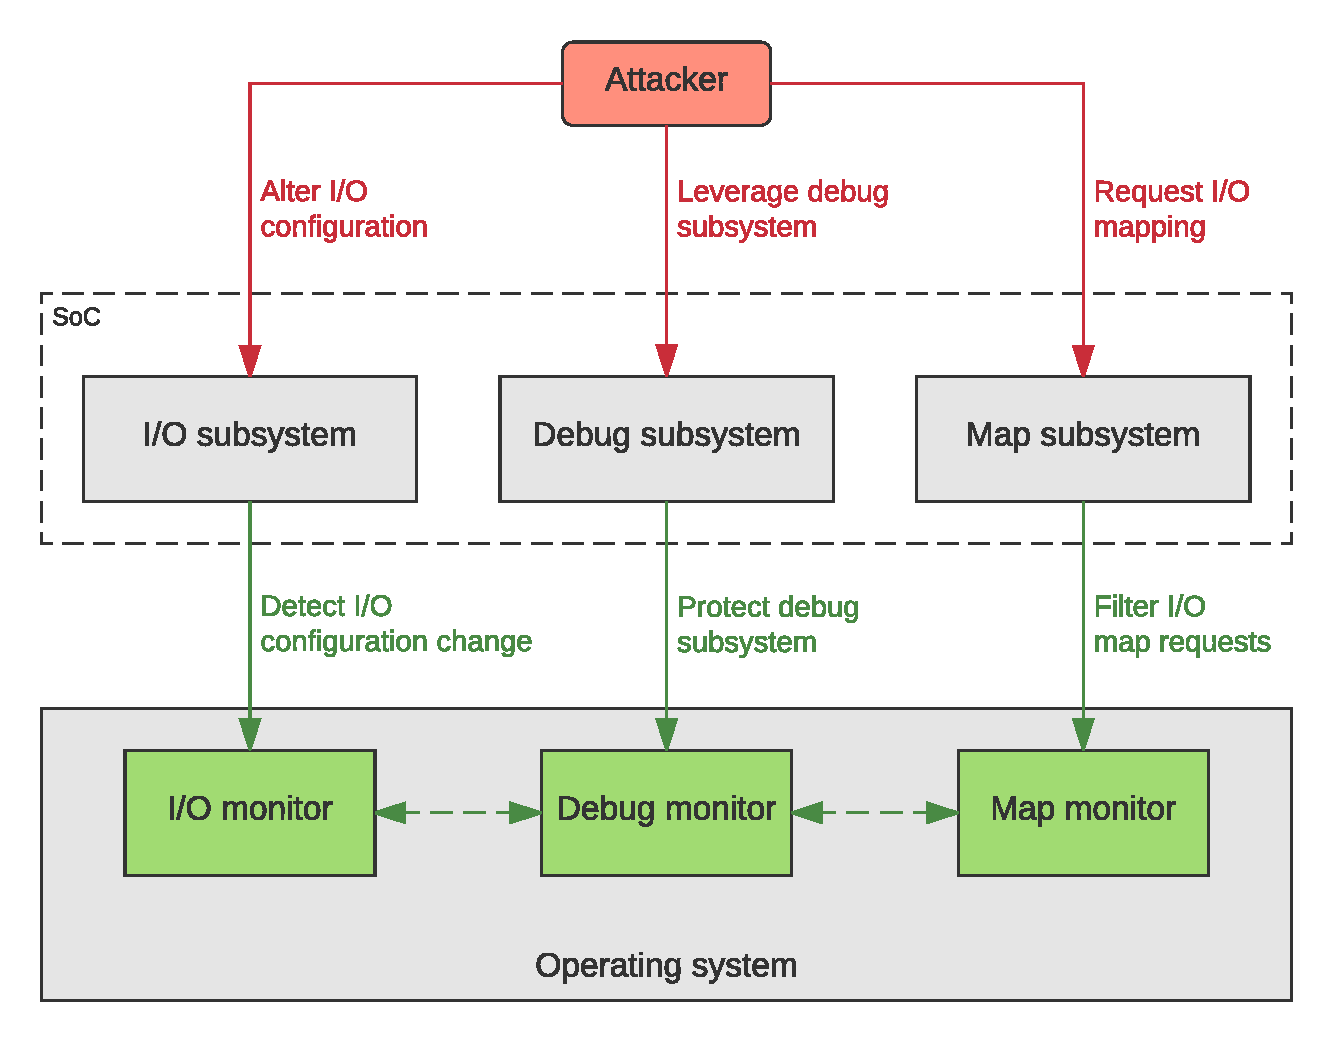
\includegraphics[width=0.8\textwidth]{res/defense}}
\caption{Pin Control Defense general architecture \label{fig:defense}}
\end{figure}
Considering that the attacker can possibly follow any of the paths highlighted in red in the figure,
our monitoring system has been divided into three main components:
\begin{itemize}
	\item \itemname{I/O monitor}: its purpose is to watch the I/O configuration, detect and react to any malicious change.
	\item \itemname{Debug monitor}: it aims to protect the debug subsystem from malicious usage.
	\item \itemname{Map monitor}: it acts as a filter for mapping requests targeting I/O memory.
\end{itemize}

Each monitor is responsible for reporting detection information related to any interesting event of the respective subsystem,
and reacting to these events according to its own configuration. The events are not necessarily due to Pin Control Attack,
\eg an I/O configuration change event may be caused by the PLC runtime.
Therefore, the I/O monitor should decide whether a particular I/O modification can be considered legitimate or not.
Debug and map monitors, instead, serve at least the following purposes:
\begin{itemize}
	\item \itemname{early detection}: the attack can be detected before it modifies the I/O configuration;
	\item \itemname{raising the bar}: they limit the attacker possibilities, by restricting the access to the corresponding subsystem;
	\item \itemname{reporting info}: they provide additional information, useful to figure out how an eventual attack has been conducted.
\end{itemize}
Since these modules are designed to be customisable, the actual effects depends on their configuration.
The following sections describe in more detail the design and the role of each module.


\subsection{I/O monitor}
\label{sec:io-design}

The I/O monitor plays the most critical role into our detection system.
Its main task is to cyclically check the values contained into I/O configuration registers, to verify that they are conforming with the logic currently loaded into the PLC.
If a change into a target register has been detected, it determines whether this modification is legal or not, according to a given trusted behaviour.
As discussed in \mysec{sec:plc-arch}, a new I/O configuration may come with a new PLC logic, and the PLC runtime must be able to apply the change without
having our defense to interfere.
Therefore, an automated mechanism able to distinguish between trusted and malicious configurations is needed.
This is not an easy problem, because an optimal solution would require an authentication between PLC runtime and I/O subsystem,
and this is not reasonable in our highly constrained system.

To tackle this problem, we designed the following strategy, which we used to implement the I/O monitor:
\begin{enumerate}
	\item define I/O configuration registers;
	\item define a trusted behavioural model of the I/O configuration;
	\item \label{enum:io-monitor} constantly monitor the I/O configuration to detect possible modifications;
	\item if a change is detected, verify whether it is conforming to the defined behaviour or not;
	\item if it is, accept the new configuration and go back to \ref{enum:io-monitor};
	\item otherwise, it is probably I/O Attack: react according to the configured monitor action and go back to \ref{enum:io-monitor}.
\end{enumerate}
The first step is to choose which registers should be included into the I/O configuration, \ie which registers should be protected.
This set of registers includes, ideally, all the registers whose modification may produce an effect on the physical process.
However, it is not always possible to define a behavioural model or enable the protection for each register. For instance,
some registers may be write-only (\eg pull-up/down registers), and there is no way to verify their current value.
Whether to include or not a register into I/O configuration should be decided case by case,
according to the protection feasibility and the possible effects of a malicious modification.

To define the behavioural model, it is required to determine the set of configuration registers actively used into the target system,
\ie the set of registers that may affect the physical process. Then, for each register (or for each bit of each register if necessary),
the model should define under which conditions the corresponding value may change. These conditions are highly dependent on the target implementation.
Generally speaking, they can be represented by simple time constraints (\eg the value cannot change twice within $\SI{20}{ms}$),
logical conditions (\eg the value must be conforming to the running PLC logic), a statistical model, or a combination of these.
Each condition can either provide an exact distinction between a trustworthy and a malicious modification (typically logical conditions),
or a heuristic only. For this purpose, we analyse in more detail the proposed logical condition, since it is able to completely exclude false positives.
The condition states that a change can be accepted only if the new I/O configuration is in line with the operations performed by the running PLC logic
(see \mysec{sec:io-impl} for more details).
Checking this condition is feasible as long as enough knowledge of the PLC runtime is available. To obtain this knowledge, two ways are doable:
\begin{itemize}
	\item \itemname{reverse engineering}: by analysing the PLC software it is possible to dynamically obtain the required information from the running logic;
	\item \itemname{PLC runtime vendor collaboration}: if the PLC software is designed to be aware of the defense mechanism,
		it could better expose the required information to the I/O monitor at run-time, thus removing the need for reverse engineering.
\end{itemize}
Once the I/O monitor is able to determine which operations the PLC logic is carrying on, it can easily decide if an I/O configuration is malicious or not,
and can effectively detect Pin Control Attack (see our approach in \mysec{sec:io-impl}).
Note that, if the information on the current I/O operations is made available by the PLC runtime, the attacker can modify it as well while conducting the attack.
In this case, however, the attacker needs to modify the PLC logic, and this may be easily noticed if further protection mechanisms are provided by the PLC runtime
(see \mysec{sec:def-sec}). Therefore, the attack would lose one of the features that made it stealth.
Moreover, from our experiments, we found that the PLC programming software typically does not perform any check about the I/O configuration.
For instance, it is possible to upload a new PLC logic together with an I/O configuration which is in conflict with the logic itself.
Thus, our approach could also be useful to detect not only I/O attacks, but any conflict between the actual I/O configuration and the expected behaviour of the logic.

An important parameter to discuss is the time interval of the main monitor loop. Since no other mechanisms are provided by the hardware,
such as interrupts, we can only detect I/O configuration changes by cyclically checking its current values. Greater scanning intervals may give the attacker
enough time-window to reach its purpose. For instance, given a PLC scan cycle of $\SI{10}{ms}$ and a monitor interval of $\SI{50}{ms}$,
if the attack is able to synchronise itself with the monitor loop, it has enough time to alter $\left \lfloor{\frac{\SI{50}{ms}}{\SI{10}{ms}}}\right \rfloor = 5$
consecutive I/O operations and then restore the configuration back before getting noticed. Smaller intervals, instead, may cause too much performance overhead.
We provide our experimental results in \mychap{chap:results}.

Another challenging aspect of this approach is to decide which action the monitor should follow if an attack has been detected.
We distinguished at least three main reactions for I/O monitor:
\begin{itemize}
	\item report the event to the system;
	\item revert the configuration back to the last known before the attack;
	\item stop the control process.
\end{itemize}
The choice among these actions (or a combination of them) again depends on the target implementation.
Typically, reporting the event is the minimum that the monitor can do, while other reactions should be decided according to risk associated with the physical process
and to the monitor reliability. If a detection is proven to be correct, due to an exact condition,
then reverting the configuration back could be the best choice. Otherwise, if the detection condition is a heuristic and the risk is critical,
stopping the control process may be considered as a more cautious alternative.
In general, if a monitor only reports about events we call it \emph{passive}, otherwise it is an \emph{active} monitor.


\subsection{Debug monitor}
\label{sec:dr-design}

This monitor is responsible for protecting the debug subsystem from malicious usage. Debug registers may be used by the attacker to gain accurate timing
information about the PLC logic I/O operations.
Similarly to what the I/O monitor does, the debug monitor continuously watches the values contained into debug registers to detect malicious modifications.
In our design, we assumed that there is no need to use debug registers into the target PLC if it is already deployed into a real control system.
As confirmed by our experiments, they are actually never used.
Typically, the SoC debug subsystem may only be needed by PLC vendors during design and implementation of their own product.
Since the operating system may provide user level access to debug registers (\eg \verb|ptrace| API on Linux), we can simply disable this user interface.
However, there is no mechanism to permanently disable debug registers also at kernel-wide level.
To understand this problem, we need to distinguish the following two cases: the debug support can be either enabled or disabled into the kernel itself.
If it is enabled, the attacker may simply leverage the system interface to use debug registers from kernel space.
If debug support is disabled, an attacker who gains kernel level access (as in kernel module version of Pin Control Attack) can always re-enable them at run-time
by inserting its own debug exception handler into the OS interrupt vector table (see \cite{arm-evt,x86-idt}).
However, this kind of attack is already covered by the defenses assumed in our threat model, because it is a data hooking technique.
Thus, we designed the following monitor strategy, that is required only if debug support is enabled into the operating system:
\begin{enumerate}
	\item disable debug registers user space interface;
	\item \label{enum:debug-monitor} constantly monitor debug registers to detect possible modifications (from kernel space);
	\item if a change is detected, it is I/O Attack: react according to the configured monitor action and go back to \ref{enum:debug-monitor}.
\end{enumerate}
The strategy is (in part) a simplification of the I/O monitor approach, on which the trusted behavioural model assumes that debug registers never change in a production system.
Based on this assumption, the debug module allows our defense to provide an early detection of the attack, before I/O configuration is actually altered.
The discussion about the monitor time interval is the same as for the previous I/O monitor: a trade-off between attacker time-window and monitor overhead.

When an attack has been detected, restoring the previous values of debug registers is surely the best action to take,
because the assumption ensures that only malicious changes may occur.
Halting the PLC process, instead, is certainly not needed because the control process is not directly affected by a modification of the debug subsystem.
In any case, the event is reported to the system. To uniform the design, the debug monitor can be configured either as passive or active,
although the passive mode is strongly discouraged for the above reasons. If the monitor is active, it actually raises the bar for the attacker,
who cannot leverage debug registers anymore.


\subsection{Mapping monitor}
\label{sec:map-design}

As discussed in \mysec{sec:pre-analysis}, the attacker may either request a new mapping between physical and virtual memory, or re-use an existing one before
modifying I/O configuration. The map monitor leverages this fact, providing a further detection mechanism usable in combination with the previous two.
Typically, the operating system provides an interface, for user space, through which each process can map a physical address region to a corresponding virtual region.
In the following part of this document we refer to it as ``mapping interface''.
The actual mapping is performed inside the kernel, and the process receives a valid virtual address as result.
The attacker can leverage this mechanism to gain access to the I/O configuration registers from user space.
According to the implementation, the PLC runtime may use this mechanism as well, and if it does, the attacker may try to re-use the PLC runtime virtual address.
We distinguish at least two techniques to re-use existing virtual addresses:
\begin{itemize}
	\item exploit a remote code execution vulnerability on the PLC runtime owning the addresses;
	\item set debug register on PLC runtime virtual address (the debug handler will have access to the process virtual addresses).
\end{itemize}
We exclude the second technique, because it is already detectable by the debug monitor. The first one, instead, can only be counteracted by detecting the control flow attack itself.
Thus, the aim of this monitor is not to detect addresses re-using, which is out of our scope, but to monitor \emph{new} mapping requests.
To achieve the goal, we dynamically replace the functions belonging to the mapping interface with our own versions (hook).
We can summarise the strategy of the map monitor as follows:
\begin{enumerate}
	\item \label{enum:map-model} define a trusted behavioural model for I/O mapping requests of the PLC runtime;
	\item hook all the functions belonging to the mapping interface;
	\item at each new mapping request, verify whether the requested physical address range overlaps the I/O configuration region or not;
	\item if there is no overlap, forward the request to the original system function;
	\item if an overlapping region is detected, verify whether the request is conforming to the trusted behaviour or not;
	\item if it is, forward the request to the original system function;
	\item if it is not, it is probably I/O Attack: react according to the configured monitor action.
\end{enumerate}
The behavioural model of step \ref{enum:map-model} should describe if and how the mapping interface is used by the PLC runtime.
We analysed the behaviour of our target systems, with the following results:
\begin{itemize}
	\item Raspberry Pi: the CODESYS runtime un-maps and re-maps the I/O every time a new PLC logic is uploaded;
	\item Wago PLC: e!RUNTIME never maps physical I/O from user space, because it is managed by the system driver.
\end{itemize}
The next step of the strategy, function hooking, must satisfy at least the following requirements (see implementation in \mysec{sec:def-impl} for more details):
\begin{itemize}
	\item it must be efficient: mapping functions may be called many times by processes (\eg in Linux, they are used not only to map physical memory,
		but any file, device, etc.);
	\item considering the threat model discussed in \mysec{sec:threat-model}, it must be applied before the Autoscopy Jr. detection system is deployed;
		otherwise, our modification will be considered as malicious.
\end{itemize}

Finally, the reaction of the map monitor to an eventual detection depends on the PLC runtime behaviour. If the PLC runtime maps the I/O (as in Raspberry Pi),
then a mechanism to distinguish between good and malicious requests is needed. To accomplish this, we may list the following alternatives:
\begin{itemize}
	\item heuristic approach based on statistical data;
	\item integration of the defense with the PLC runtime.
\end{itemize}
Since the first approach cannot give an exact detection, the monitor may simply report the detection to the system.
The second approach, instead, may be implemented in different ways. For instance, the map monitor could provide a separate mapping interface
reserved only for the PLC runtime process.
In any case, if the system allows to have an exact detection mechanism, the monitor may directly deny the malicious request, factually raising the bar for the attacker.


\section{Implementation}
\label{sec:def-impl}

We describe here our implementation of the above strategies, discussing the engineering problems encountered and the adopted solutions.
Since the authors of the attack presented their work as ``Ghost in the PLC'' \cite{ghostplc}, we called our defense prototype implementation \emph{Ghostbuster}.
Ghostbuster is a kernel module written in C language, targeting Embedded Linux running on ARM architecture.
It is designed to be highly configurable and as architecture-independent as possible, following the guideline of the Linux kernel itself.
A portion of the code, \ie the lowest level code, is still dependent from the specific architecture (\eg ARM), but is separated from the general implementation template.
This allows Ghostbuster to be easily extendable to other architectures and SoCs running Linux. At the same time, we focused on maintaining the lowest overhead possible,
which is always crucial for PLCs. We proceed with the description of the overall architecture, and then we go deep into each module of the architecture.
Finally, we describe the usage of our kernel module.


\subsection{Implementation architecture}

The implementation architecture is based on the general one described in \mysec{sec:def-arch}. Thus, we implemented I/O, debug and map monitors.
Each one of them has been divided into two main parts, following the template method pattern: the main strategy and the sub-actions implementation.
The aim of this separation is to minimise the effort needed to deploy our defense into different systems, thus improving its portability.
In particular, we considered the following variables: each target system may have its own System on Chip, firmware and PLC runtime.
During the design part, we defined high-level monitor strategies, which allowed us to provide an abstraction adaptable to any Linux-based system,
independently from these variables.
\begin{figure}[h]
\centerline{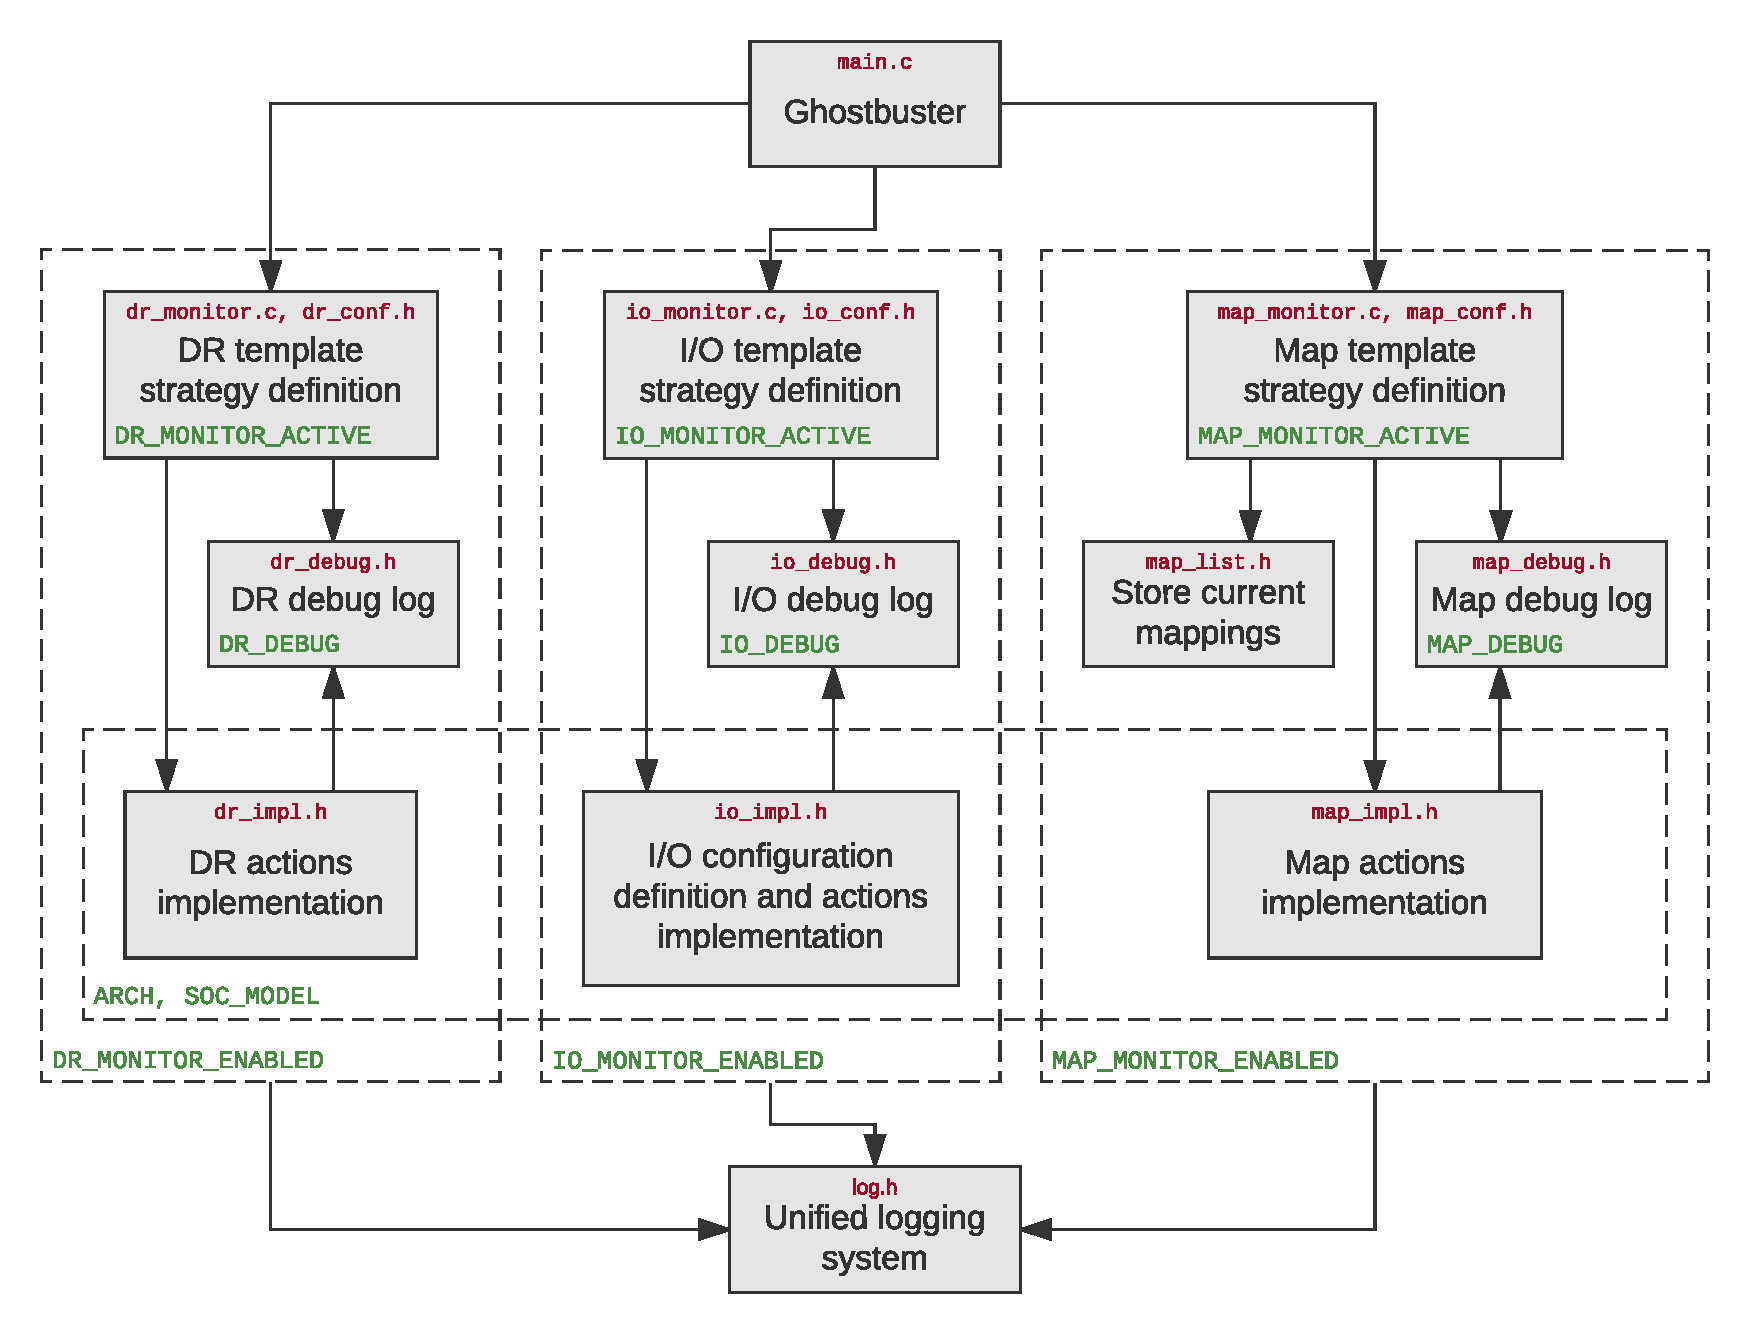
\includegraphics[width=\textwidth]{res/def-impl}}
\caption{Ghostbuster implementation architecture \label{fig:def-impl}}
\end{figure}

The resulting architecture is shown in \myfig{fig:def-impl}, which associates each specific role to the corresponding source file(s) (in red).
Furthermore, the compilation of our module can be parameterised in different ways, as shown by the green labels in the figure.
Each green label, associated to a rectangle container in the figure, corresponds to a compiler flag or parameter that affects the compilation of the enclosed portion,
either enabling/disabling the component or changing its default behaviour.
The compilation is managed by a \verb|Makefile|, in which all the required flags are defined and passed to the compiler.
The \verb|Makefile| needs to know the location of the target Linux kernel source directory, in order to link Ghostbuster with the kernel code.

In particular, each monitor can be enabled or disabled by means of the following flags:
\begin{Verbatim}[fontsize=\small]
	IO_MONITOR_ENABLED
	DR_MONITOR_ENABLED
	MAP_MONITOR_ENABLED
\end{Verbatim}
If a monitor is disabled, it will not be included into the compilation at all, reducing the final binary size.
This may be useful to exclude a particular monitor that is not needed by the target system
(\eg DR monitor if debug support is not enabled into the kernel, see discussion in \mysec{sec:dr-design}).

When a monitor is enabled, its execution mode may be controlled by one of the following flags, respectively:
\begin{Verbatim}[fontsize=\small]
	IO_MONITOR_ACTIVE
	DR_MONITOR_ACTIVE
	MAP_MONITOR_ACTIVE
\end{Verbatim}
If one of these flags is not defined, the corresponding monitor is compiled in \emph{passive} mode: it will only reports about events, without taking any further action.
Otherwise, the monitor is \emph{active} and it will include its specific reactions to the events.
If a monitor is disabled, the corresponding active flag is ignored.

The messages reported by each monitor may be extended by enabling the following debug flags:
\begin{Verbatim}[fontsize=\small]
	IO_DEBUG
	DR_DEBUG
	MAP_DEBUG
\end{Verbatim}
If a debug flag is defined, the corresponding monitor will print out its complete state at each event detection.

Finally, the \verb|ARCH| and \verb|SOC_MODEL| variables are used to select a specific implementation for the enabled monitors.
An implementation is identified by an architecture name and a SoC model (\eg \verb|arm|, \verb|BCM2835|). Given this information,
the implementation files will be automatically included from the \verb|<ARCH>/<SOC_MODEL>/| sub-directory.
We chose to directly include the implementation part into header files, instead of external compilation units (\verb|.c| files), to allow the usage of \verb|inline|
functions. The code of an inline function is directly included into the caller, and it does not need an explicit function call.
This may cause some code duplication, which we tried to minimise, but it achieves better performance,
especially for those functions that are called many times (\eg in the main loop of a monitor).

When Ghostbuster is loaded, the three main monitors are started in parallel.
The monitors are independent from each other, and every monitor has its own kernel thread.
When a monitor has to report an event to the system, it uses the common logging subsystem available into the kernel
(see \mysec{sec:def-usage} for more information).
The target systems used to test our defense are exactly the same as the ones described for the attack part in \mychap{chap:attack}, with the same PLC logic and I/O configuration.
In particular, for each monitor, we first refer to the Raspberry Pi system (BCM2835 SoC); then we discuss the modifications required to run on Wago PLC as well.
In the following sections we describe in more detail the structure and the operations performed by each monitor.
From now on, we will refer to the abstract part of each monitor as the \emph{interface}, and to the architecture-dependent part as the \emph{implementation}.


\subsection{I/O monitor}
\label{sec:io-impl}

This monitor is responsible for protecting I/O configuration memory from malicious usage.
The monitor interface includes the I/O configuration data type, modeled as a set of memory blocks by means of the \verb|io_conf_t| structure:
\begin{lstlisting}
typedef struct {
	const void** addrs; // Set of block base addresses
	const unsigned* sizes; // Size of each block in bytes
	const unsigned blocks; // Number of blocks
	const unsigned size; // Total size in byte
} io_conf_t;
\end{lstlisting}
This model takes into account the fact that I/O registers may be located at different addresses, resulting in a non-contiguous I/O memory.

With reference to the BCM2835 manual \cite{bcm2835} and to the target configuration defined in \mysec{sec:attack-pi},
we defined, into the implementation part, the set of I/O registers we want to protect.
In particular, since our system uses GPIO pins, two of which multiplexed to I2C, we chose to protect GPIO pin control registers, whose physical base address is \verb|0x2020000|.
These registers are responsible both for pin configuration and pin multiplexing. Each register is 32-bit wide, having 3 bits for each I/O pin: it can control $10$ different pins.
Although our target system uses only four pins for its I/O, to be more general, we decided to protect all the available GPIO pins ($54$).
Hence, we included all $6$ pin control registers into the definition of our I/O configuration, by filling in the \verb|io_conf_t| global structure:
\begin{lstlisting}
#define IO_BLOCKS            	1 // Registers are contiguous: one block needed
#define PIN_CTRL_BASE        	((void*)0x20200000) // Pin control base address
#define PIN_CTRL_SIZE        	24 // 6 regs * 4 bytes each
#define __IO_STATE_TOTAL_SIZE	24 // Total size in bytes

static const void* bcm2835_io_addrs[IO_BLOCKS] = { PIN_CTRL_BASE };
static const unsigned bcm2835_io_sizes[IO_BLOCKS] = { PIN_CTRL_SIZE };

static const io_conf_t phys_io_conf = {
	.addrs = bcm2835_io_addrs,
	.sizes = bcm2835_io_sizes,
	.blocks = IO_BLOCKS,
	.size = __IO_STATE_TOTAL_SIZE
};
\end{lstlisting}
Of course our implementation is only a prototype, and many other registers may be included into the I/O configuration (\eg event detect, edge detect, I2C control registers, etc.).

The next step is to define the trusted behaviour of the I/O configuration.
In particular, we have pin multiplexing (\emph{pinmux}) and pin configuration (\emph{pinconf}) registers, and we assumed the following behaviour:
\begin{itemize}
	\item \itemname{pinmux registers}: they are initialised at boot time, and never change during run-time;
	\item \itemname{pinconf registers}: they are initialised at boot time, but can be modified at any time by the PLC runtime, maintaining the following invariant:
		every pin configuration (input or output mode) must be conforming to the running PLC logic.
\end{itemize}

After I/O configuration has been defined, we can describe the interface and implementation of the I/O monitor.
The abstract part is essentially made of the monitor loop, which executes the main strategy,
and the detection handler, called by the implementation when an I/O modification has been detected. Both codes are shown in \myalg{alg:io-iface},
and they are independent from any specific architecture or SoC model.
\algnewcommand\True{\textbf{true}\space}
\algnewcommand\False{\textbf{false}\space}
\algnewcommand\algorithmicforeach{\textbf{for each}}
\algdef{S}[FOR]{ForEach}[1]{\algorithmicforeach\ #1\ \algorithmicdo}
\begin{algorithm}[h]
\caption{I/O monitor interface: main loop and detection handler}
\label{alg:io-iface}
\begin{algorithmic}[1]
\Function{IOMainLoop}{\null}
	\State $t \gets$ monitor scan interval \Comment{The monitor interval in $\SI{}{ms}$}
	\State $C \gets$ physical I/O configuration \Comment{The defined I/O configuration}
	\State $T \gets$ \Call{GetIOState}{$C$} \Comment{Read trusted state from I/O registers}
	\Loop
		\ForEach{block $B \in C$ having index $i$}
			\State \Call{CheckIOState}{$B, T[i]$} \Comment{Compare current and trusted state of block $B$}
		\EndFor
		\If{monitor should stop}
			\State \Return \Comment{Return if Ghostbuster is being stopped}
		\EndIf
		\State \Call{msleep}{$t$} \Comment{Wait for next cycle}
	\EndLoop
\EndFunction
\Statex
\end{algorithmic}

\begin{algorithmic}[1]
\Function{HandleIODetection}{$D$} \Comment{React to the detection $D$}
	\State report about D
	\If{I/O debug enabled}
		\State dump entire I/O state
	\EndIf
	\If{\Call{IsLegitimate}{$D$}}
		\State \Call{UpdateIOState}{$D$} \Comment{Accept new configuration, update trusted state}
	\Else
		\State report about I/O Attack
		\If{I/O monitor is active}
			\State \Call{RestoreIOState}{$D$} \Comment{Reject new configuration, restore trusted state back}
		\EndIf
	\EndIf
\EndFunction
\end{algorithmic}
\end{algorithm}

Each iteration of the main loop is executed every $t~\SI{}{ms}$, where the specific value of $t$ is defined into the \verb|IO_MONITOR_INTERVAL| flag.
The loop terminates only if an external signal indicates that Ghostbuster is being stopped (see \mysec{sec:def-usage}).
The verification of the current I/O configuration is performed at block level against the golden reference, which is obtained by \textproc{GetIOState} before starting the loop.
Since we assume that the system is in a safe state when our module is deployed, the initial I/O state read from configuration registers is considered trusted.
When a modification is detected by \textproc{CheckIOState}, the detection handler is called back and the monitor strategy is applied.
Note that the handler may be called many times from the same call to \textproc{CheckIOState}, because there may be more than one single modification within one contiguous block.
The detection granularity is decided by the implementation part (\eg for each single pin in our implementation).
If the modification is considered legitimate, then the reference I/O state is updated with the new configuration.
Otherwise, we report the attack to the system and, since we have an exact detection condition which cannot give false positives,
we may safely restore the previous configuration back if the I/O monitor is in active mode.

All the low-level I/O functions are defined into the implementation part, and may be different for each target system.
\begin{algorithm}[h!]
\caption{I/O monitor implementation functions}
\label{alg:io-impl}
\begin{algorithmic}[1]
\Function{GetIOState}{$C$} \Comment{Read current I/O state}
	\State $T \gets \emptyset$
	\ForEach{block $B$ in $C$}
		\ForEach{register $R \in B$}
			\State $T \gets T \cup \Call{ioread32}{$R$}$ \Comment{Save value of register $R$ into the trusted state}
		\EndFor
	\EndFor
	\State \Return $T$
\EndFunction
\Statex
\end{algorithmic}

\begin{algorithmic}[1]
\Function{CheckIOState}{$B, T_B$} \Comment{Verify block $B$ against its trusted state $T_B$}
	\ForEach{register $R \in B$ having index $i$}
		\State $C_R \gets \Call{ioread32}{$R$}$ \Comment{Read current value of register $R$}
		\State $T_R \gets T_B[i]$ \Comment{Trusted value of register $R$}
		\ForEach{pin $p \in R$ having index $j$}
			\State $d \gets C_R[j] \oplus T_R[j]$ \Comment{Difference between current and trusted value}
			\If{$d \neq 0$}
				\State $D \gets \{C_R, T_R, j, d\}$ \Comment{Fill in detection information}
				\State \Call{HandleIODetection}{$D$} \Comment{Call detection handler}
			\EndIf
		\EndFor
	\EndFor
\EndFunction
\Statex
\end{algorithmic}

\begin{algorithmic}[1]
\Function{IsLegitimate}{$D$}
	\If{$D$ is pin multiplexing}
		\State \Return false \Comment{Pin multiplexing is not allowed at run-time}
	\EndIf
	\If{$D$ is pin configuration}
		\If{new I/O configuration is conforming to PLC logic}
			\State \Return true \Comment{Change performed by the PLC runtime}
		\Else
			\State \Return false \Comment{Malicious change}
		\EndIf
	\EndIf
\EndFunction
\Statex
\end{algorithmic}

\begin{algorithmic}[1]
\Function{UpdateIOState}{$D$}
	\State $D.T_R[j] = D.C_R[j]$ \Comment{Update the trusted value according to new I/O configuration}
\EndFunction
\Statex
\end{algorithmic}

\begin{algorithmic}[1]
\Function{RestoreIOState}{$D$}
	\State \Call{iowrite32}{$D.T_R \oplus D.d$} \Comment{Restore I/O configuration to the trusted value}
\EndFunction
\end{algorithmic}
\end{algorithm}
These functions deal with the effective accesses to I/O registers, which depend on many factors.
The implementation knows the way to access these registers, their size and their bits arrangement.
In \myalg{alg:io-impl} we show our implementation related to the BCM2835 SoC, where all registers are 32-bits wide.

The detection events are managed at pin level, \ie if an attacker modifies the configuration of more than one pin at a time, only one pin at a time is verified.
The critical function of the implementation part is the \textproc{IsLegitimate} function, which decides whether a configuration change is legal or not.
Based on our behavioural model, pin multiplexing can never be legitimate during run-time, so the implementation is straightforward.
In the case of pin configuration, instead, the implementation needs to check if the I/O configuration after the change is in conflict with the PLC logic.
A conflict occurs in one of the following two cases:
\begin{itemize}
	\item \itemname{write}: the pin is set as input and the logic is trying to write from it;
	\item \itemname{read}: the pin is set as output and the logic is trying to read from it.
\end{itemize}
The most challenging problem here is to figure out which operation the logic is performing on a given I/O pin.
To solve this problem, we applied the reverse engineering approach proposed in \mysec{sec:io-design}, reported below. 

Inside the BCM2835, a specific set of 32-bit registers is used to interact with I/O pins: LVL registers to read the pin value,
CLR registers to write a $0$ and SET registers to write a $1$ \cite{bcm2835}. Every register contains a bit for each pin, for a total of 32 pins per register.
To have access to the operations performed by the PLC logic on these registers, we leveraged the debug subsystem.
In ARM architecture, the debug subsystem provides two different types of debug registers: breakpoint and watchpoint (see \mysec{sec:dr-impl}).
When a pin configuration change is detected, the I/O monitor inserts a watchpoint to the corresponding LVL, CLR or SET register of the affected pin,
in order to intercept the I/O operation performed by the PLC logic. The watchpoint can be set for either a read or a write, according to the specific case we want to verify.
From a reverse engineering analysis of the PLC runtime, we found that read and write operations are performed with the following instructions, respectively:
\begin{itemize}
	\item \verb|STR R2, [R3]| (Opcode \verb|0x002083E5|, \verb|R3| contains the address of a STR or CLR register);
	\item \verb|LDR R2, [R3]| (Opcode \verb|0x002093E5|, \verb|R3| contains the address of a LVL register).
\end{itemize}
\verb|R3| always contains the virtual address targeted by our watchpoint. When a watchpoint is hit, the debug exception handler is called,
and all the execution context of the process is passed as argument. Inside the debug handler, we proceed as follows, according to the case:
\begin{itemize}
	\item \itemname{write}: we look at the content of \verb|R2| to check if the PLC logic is trying to write to the specific pin changed to input.
		If \verb|R2| contains a $1$ corresponding to the target pin, then we can conclude that the new configuration is in conflict with the logic.
	\item \itemname{read}: in this case more reverse engineering of the PLC runtime is needed to know which pins (\ie bits) are actually used by the logic as input,
		because the instruction always loads the entire register (32 pins).
		To simplify the detection in our prototype version, we supposed that the PLC logic may only have one input pin for each register.
		In this case, reading from the register implies that the PLC logic is trying to read from the given pin. Thus, we can report a conflict.
		To remove this assumption, which limits the applicability of our defense, more knowledge about the PLC runtime is required.
		As previously discussed, this knowledge can be obtained either from a deeper reverse engineering analysis or from a collaboration with the PLC runtime vendor.
		For instance, each PLC logic may be designed to contain a constant bit mask having one bit for each pin,
		where each bit specifies whether the corresponding pin is currently used as input or output. If such data was available,
		the I/O monitor could look at it instead of inserting a watchpoint and looking for the actual operations.
		This mechanism raise the bar for the attacker, who would need to alter the PLC logic code as well to conduct the attack,
		thus defeating its stealthiness.
\end{itemize}

Note that from a performance perspective our approach is feasible, because it inserts a debug exception only in case of an I/O modification to determine if it is malicious.
Thus, this may cause an overhead when a good I/O configuration is updated by the PLC runtime as well. See \mychap{chap:results} for more details about our results.

Besides its main functions, the I/O monitor provides an additional interface, which is needed by the MAP monitor.
When the MAP monitor has to filter mapping requests coming from system processes, it needs to know whether a request of a physical address range includes
at least one address belonging to the I/O configuration. This is provided by the I/O monitor with the function listed in \myalg{alg:io-overlap},
which accepts a pair of physical addresses $[s, e]$ representing the start and the end addresses of the given range.
\begin{algorithm}[h]
\caption{I/O monitor overlap function}
\label{alg:io-overlap}
\begin{algorithmic}[1]
\Function{MapOverlapsIO}{$s, e$} \Comment{Check if physical range $[s, e]$ overlaps I/O configuration}
	\State $C \gets$ physical I/O configuration \Comment{The defined I/O configuration}
	\ForEach{block $B$ in $C$}
		\If{$(B.s \le s \le B.e) \lor (B.s \le e \le B.e)$} \Comment{Overlap condition at block level}
			\State \Return \True
		\EndIf
	\EndFor
	\State \Return \False
\EndFunction
\end{algorithmic}
\end{algorithm}
Since this function is needed by the MAP monitor independently from I/O monitor operations, we designed it to be available even if the I/O monitor is disabled.
The I/O configuration, needed by \textproc{MapOverlapsIO}, is made available independently from the I/O monitor as well.
Note that, there might exist some target systems in which disabling the I/O monitor has sense. For instance, consider a system having the following two properties:
\begin{itemize}
	\item the root/kernel access is properly protected (\eg kernel protected by execute only memory or TrustZone),
		or it has sufficient security level for which is not worth to insert the I/O monitor (\eg no admin default passwords, hardened kernel, etc.);
	\item the PLC runtime, or any other process, does not use the mapping interface (\ie on Wago PLC).
\end{itemize}
On such a system, the MAP monitor alone could be enough to protect the I/O configuration, because it can simply deny any access to I/O physical addresses from user space,
while the system itself is already protected from kernel space accesses.


\subsubsection{Wago PLC version}

To port the I/O monitor to the Wago PLC system, only the following changes are necessary:
\begin{itemize}
	\item \itemname{I/O configuration}: the I/O configuration and the behavioural model must be redefined according to the registers used by the Wago PLC.
		In particular, the implementation may include pin configuration and pin multiplexing registers as well, plus SPI, DMA and IRQ registers.
		The way to access registers is pretty much equal to the Raspberry Pi system, because are both ARM architectures with 32-bit wide registers.
		On Wago PLC, pin configuration and pin multiplexing are managed by two different set of registers. Therefore, the low-level implementation
		is even simplified, because it does not need to distinguish configuration and multiplexing bits inside registers.
		However, including other registers (\eg SPI, DMA, IRQ, etc.) may lead to more complex behavioural models which need to be analysed.
	\item \itemname{Debug subsystem}: given the engineering problem described later in \mysec{sec:dr-impl}, the same solution using watchpoint cannot be directly applied.
		To get the needed information about the PLC logic, two ways are possible. Either the debug interface is implemented into the kernel for AM3517 SoC,
		or a better integration with the PLC runtime is required, as already discussed.
\end{itemize}


\subsection{DR monitor}
\label{sec:dr-impl}

The DR monitor aims to protect the debug subsystem. As described for the design phase, the DR monitor needs to accomplish two goals:
\begin{itemize}
	\item disable debug interface access from user space;
	\item watch over debug registers value to detect malicious events.
\end{itemize}

In Linux, the debug user interface is based on the following functions \cite{hw-breakpoint}:
\begin{lstlisting}
struct perf_event* register_user_hw_breakpoint(struct perf_event_attr* attr,
                                               perf_overflow_handler_t handler,
                                               struct task_struct* tsk);

int modify_user_hw_breakpoint(struct perf_event *bp,
                              struct perf_event_attr *attr);

void unregister_hw_breakpoint(struct perf_event *bp);
\end{lstlisting}
To disable these functions, we dynamically patched the kernel text replacing the prologue instructions of each function.
In particular, they have the following prologue:
\begin{Verbatim}[fontsize=\small]
	c00d3cb0 <register_user_hw_breakpoint>:
	c00d3cb0: e1a0c00d  mov  ip, sp
	c00d3cb4: e92dd800  push {fp, ip, lr, pc}
	c00d3cb8: e24cb004  sub  fp, ip, #4
	c00d3cbc: e24dd008  sub  sp, sp, #8
	[...]

	c00d3e30 <modify_user_hw_breakpoint>:                                
	c00d3e30: e1a0c00d  mov  ip, sp
	c00d3e34: e92ddff0  push {r4, r5, r6, r7, r8, r9, sl, fp, ip, lr, pc}
	c00d3e38: e24cb004  sub  fp, ip, #4
	c00d3e3c: e24dd00c  sub  sp, sp, #12
	[...]

	c00d3ce8 <unregister_hw_breakpoint>:
	c00d3ce8: e1a0c00d  mov   ip, sp
	c00d3cec: e92dd800  push  {fp, ip, lr, pc}
	c00d3cf0: e24cb004  sub   fp, ip, #4
	[...]
\end{Verbatim}
We replaced the prologue instructions with the following ones:
\begin{enumerate}
	\item \itemname{return value}: if the function is not void (\eg in the first two cases), we need to return a value to the caller.
		Thus, we move the value \verb|-EACCES| ($-13$) into R0 by using the move-negate instruction: \verb|mvn r0, #0xC|.
		\verb|EACCES| is defined into the \verb|errno-base.h| kernel header as \verb|Permission denied|;
	\item \itemname{branch}: jump back to the caller by branching to the link register: \verb|bx lr|.
\end{enumerate}
After the patch, the kernel text becomes the following:
\begin{Verbatim}[fontsize=\small]
	c00d3cb0 <register_user_hw_breakpoint>:
	c00d3cb0: e3e0000c  mvn  r0, #0xC
	c00d3cb4: e12fff1e  bx   lr
	[...]

	c00d3e30 <modify_user_hw_breakpoint>:                                
	c00d3e30: e3e0000c  mvn  r0, #0xC
	c00d3e34: e12fff1e  bx   lr
	[...]

	c00d3ce8 <unregister_hw_breakpoint>:
	c00d3ce8: e12fff1e  bx   lr
	[...]
\end{Verbatim}

Once the user access to debug registers has been disabled, we activate the DR monitor to protect them from attackers who gain kernel access.
As for the I/O monitor, we report the interface part and the implementation.
The abstract strategy of the DR monitor is rather simple, and is listed in \myalg{alg:dr-iface}.
\begin{algorithm}[h]
\caption{DR monitor interface: main loop and detection handler}
\label{alg:dr-iface}
\begin{algorithmic}[1]
\Function{DRMainLoop}{\null}
	\State $m_T \gets$ mutex \Comment{Global mutex to protect trusted state}
	\State $t \gets$ monitor scan interval \Comment{The monitor interval in $\SI{}{ms}$}
	\State $T \gets$ \Call{GetDRState}{\null} \Comment{Read trusted state from debug registers}
	\Loop
		\State \Call{lock}{$m_T$}
		\State \Call{CheckDRState}{$T$} \Comment{Compare current and trusted state of debug registers}
		\State \Call{unlock}{$m_T$}
		\If{monitor should stop}
			\State \Return \Comment{Return if Ghostbuster is being stopped}
		\EndIf
		\State \Call{msleep}{$t$} \Comment{Wait for next cycle}
	\EndLoop
\EndFunction
\Statex
\end{algorithmic}

\begin{algorithmic}[1]
\Function{HandleDRDetection}{$D$} \Comment{React to the detection $D$}
	\If{DR debug enabled}
		\State dump entire DR state
	\EndIf
	\State report about I/O Attack
	\If{DR monitor is active}
		\State \Call{RestoreDRState}{$D$} \Comment{Restore debug register trusted state}
	\EndIf
\EndFunction
\end{algorithmic}
\end{algorithm}
It is a simplification of the I/O monitor strategy, where any modification is considered malicious.
Since in our implementation the I/O monitor makes use of the debug subsystem, the DR monitor exposes the interface listed in \myalg{alg:dr-ioiface}
to mediate any access to debug registers.
\begin{algorithm}[h]
\caption{DR monitor interface for I/O monitor}
\label{alg:dr-ioiface}
\begin{algorithmic}[1]
\Function{SetDR}{$r$} \Comment{Set a debug register $r$}
	\State \Call{lock}{$m_T$}
	\State \Call{register\_wide\_hw\_breakpoint}{$r$} \Comment{Use kernel interface for debug registers}
	\State $T \gets$ \Call{GetDRState}{\null} \Comment{Update trusted state}
	\State \Call{unlock}{$m_T$}
\EndFunction
\Statex
\end{algorithmic}

\begin{algorithmic}[1]
\Function{ResetDR}{$r$} \Comment{Reset a previously set debug register $r$}
	\State \Call{lock}{$m_T$}
	\State \Call{unregister\_wide\_hw\_breakpoint}{$r$} \Comment{Use kernel interface for debug registers}
	\State $T \gets$ \Call{GetDRState}{\null} \Comment{Update trusted state}
	\State \Call{unlock}{$m_T$}
\EndFunction
\end{algorithmic}
\end{algorithm}
By using this interface, any modification of debug registers performed by the I/O monitor is excluded from the detection.
This mechanism requires that the DR state is protected from concurrent access by a mutual exclusion mechanism.
%the interface is usable by the attacker?

All the details about debug registers are handled by the implementation part, shown in \myalg{alg:dr-impl}.
\begin{algorithm}[h]
\caption{DR monitor implementation functions}
\label{alg:dr-impl}
\begin{algorithmic}[1]
\Function{GetDRState}{\null} \Comment{Read current I/O state}
	\State $T \gets \emptyset$
	\State $D \gets hardware debug registers$
	\ForEach{debug register $r \in D$}
		\State $T \gets T \cup \Call{DRread}{$r$}$ \Comment{Save value of debug register $r$ into $T$}
	\EndFor
	\State \Return $T$
\EndFunction
\Statex
\end{algorithmic}

\begin{algorithmic}[1]
\Function{CheckDRState}{$T$} \Comment{Verify debug registers against trusted state $T_B$}
	\ForEach{debug register $r \in B$ having index $i$}
		\State $C_r \gets \Call{DRread}{$r$}$ \Comment{Read current value of register $r$}
		\State $T_r \gets T[i]$ \Comment{Trusted value of register $r$}
		\State $d \gets C_r \oplus T_r$ \Comment{Difference between current and trusted value}
		\If{$d \neq 0$}
			\State $D \gets \{C_r, T_r, r\}$ \Comment{Fill in detection information}
			\State \Call{HandleDRDetection}{$D$} \Comment{Call detection handler}
		\EndIf
	\EndFor
\EndFunction
\Statex
\end{algorithmic}

\begin{algorithmic}[1]
\Function{RestoreDRState}{$D$}
	\State \Call{DRwrite}{$D.r, D.T_r$} \Comment{Restore debug register to the trusted value}
\EndFunction
\end{algorithmic}
\end{algorithm}
The ARM architecture supports two type of hardware debug registers: breakpoints for instruction addresses, and watchpoints for data addresses.
The DR monitor protects both of them, and the detection is handled at register level. Each register is accessed through specific coprocessor instructions.
A special read-only register, the \emph{Debug ID Register} (DIDR), specifies the number of debug registers available and other useful information on the SoC configuration.
In particular, since the BCM2835 SoC supports 2 watchpoints and 6 breakpoints, the DR monitor can be deployed to protect them all.


\subsubsection{Wago PLC version}

To adapt the DR monitor for Wago PLC, the following engineering problem needs to be solved.
The AM3517 SoC model embedded into this PLC provides a different interface for debug registers. In particular, it uses a memory mapped interface
instead of specific coprocessor instructions \cite{am35x}.
Unfortunately, it turns out that this particular interface is not supported by the Linux kernel debug framework, as reported in \cite{dr-mapped}:
``The memory-mapped extended debug interface is unsupported due to its unreliability in real implementations''.
Apart from this technical problem, the DR monitor is designed to be applicable to any other ARM implementation that supports debug registers.
To port it for other architectures different than ARM, only the implementation part must be adapted.


\subsection{MAP monitor}
\label{sec:map-impl}

The purpose of the MAP monitor is to filter user space requests delivered to the mapping subsystem. On Linux, users can use the mapping interface to
map files or devices, and this mechanism can be used to map physical addresses to virtual addresses through special devices such as \verb|/dev/mem|.
Among all physical memory addresses, an attacker may be able to map specific I/O memory regions to alter I/O configuration registers.
The set of devices that can provide access to I/O physical memory depends on the specific system
(\eg for the Linux version installed on our Raspberry Pi, either \verb|/dev/mem| or \verb|/dev/gpiomem| can be used).
Linux provides the following system calls to deal with mapping requests:
\begin{lstlisting}
long mmap2(unsigned long addr, unsigned long len,
           unsigned long prot, unsigned long flags,
           unsigned long fd, unsigned long pgoff);

long mremap(unsigned long addr,
            unsigned long old_len, unsigned long new_len,
            unsigned long flags, unsigned long new_addr);

long remap_file_pages(unsigned long addr, unsigned long len,
                      unsigned long prot, unsigned long pgoff,
                      unsigned long flags);

long munmap(unsigned long addr, size_t len);
\end{lstlisting}
Note that we are describing the interface from a kernel point of view: the interface exposed to user space may be slightly different.
The \verb|mmap2| system call supersedes the old \verb|mmap|, and both use the same internal function which is \verb|sys_mmap_pgoff|.
Although these functions are used for many other types of mappings, we focus on mappings between virtual addresses and physical memory addresses.
These system calls serve the following purpose, respectively:
\begin{itemize}
	\item \itemname{mmap2}: request a new mapping related to the \verb|fd| address space (\eg \verb|/dev/mem| for physical memory) having \verb|len| bytes
		and starting from page offset \verb|pgoff|; returns the mapped virtual address pointing to the starting offset of the target address space;
	\item \itemname{mremap}: modify an existing mapping, either remapping it to a new virtual address \verb|new_addr| (\emph{move})
		or resizing it to \verb|new_len| bytes (\emph{grow} or \emph{shrink}); returns the virtual address after the modification;
	\item \itemname{remap\_file\_pages}: remap an existing mapping to point to a different start page offset \verb|pgoff| of the target address space
		(\eg to point to a different physical address); returns $0$ if successful, an error code otherwise.
	\item \itemname{munmap}: delete an existing mapping of \verb|len| bytes related to the virtual address \verb|addr|;
		the \verb|len| parameter is aligned to the next page boundary, and the resulting range of pages is removed.
\end{itemize}
The type of a requested mapping can be inferred from the \verb|fd| (file descriptor) parameter in \verb|mmap2|,
or from the \verb|addr| parameter in the other calls, which refer to previously mapped regions.
Every mapping is managed at a page level, and the arguments are aligned to page boundaries before handling the request.
The scheme in \myfig{fig:map-linux} summarises a significant sequence of operations performed via the mapping interface,
assuming physical and virtual address spaces based on $\SI{4}{\kilo\byte}$ pages.
\begin{figure}[h]
\centerline{
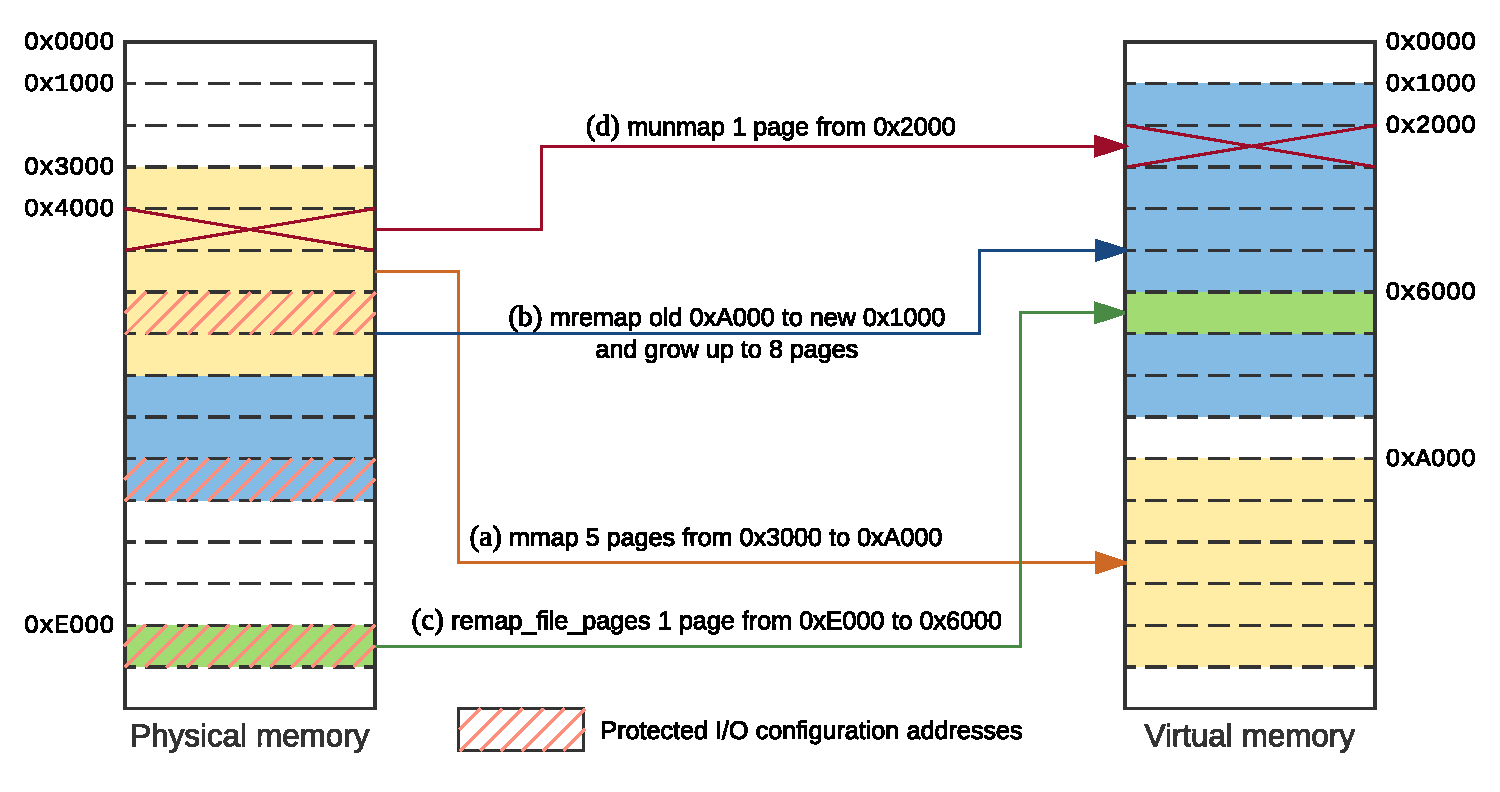
\includegraphics[width=\textwidth]{res/map-linux}}
\caption{Accessing physical addresses through Linux mapping interface \label{fig:map-linux}}
{\phantomsubcaption\ignorespaces\label{fig:mmap}}
{\phantomsubcaption\ignorespaces\label{fig:mremap}}
{\phantomsubcaption\ignorespaces\label{fig:remapfp}}
{\phantomsubcaption\ignorespaces\label{fig:munmap}}
\end{figure}
As shown in the figure, there exist $3$ different ways of accessing protected I/O physical addresses by using mapping functions.
When a mapping includes a portion (even one byte) of the I/O configuration defined by the I/O monitor, we say that an \emph{overlap} occurs.
First, an attacker may call \verb|mmap2| (or \verb|mmap|) to directly include the I/O configuration into the requested range \subref{fig:mmap}.
Second, he may use \verb|mremap| to extend a current mapping, possibly causing overlap on an I/O address which was not mapped before \subref{fig:mremap}.
Third, he can re-map an already mapped virtual address to a different physical address, including a protected I/O address as well \subref{fig:remapfp}.
Note that, the second and the third system calls identify the existing mappings by means of the virtual addresses returned by the first call to \verb|mmap2|.
Therefore, the MAP monitor must keep track of the current existing mapping (and virtual addresses) to verify if a subsequent re-map may cause an overlapping.
Finally, the \verb|munmap| call deletes an existing mapping (or part of it) \subref{fig:munmap}. Even if it cannot cause an overlap,
the \verb|munmap| system call needs to be monitored as well in order to update the data structure containing the existing mappings and remain
consistent with the kernel data structures.

To keep track of the current mappings related to physical memory, our monitor uses a global list of pages. Each page is a structure containing a physical address,
a virtual address, and a process identifier. We assume that the number of processes normally interested in physical memory is quite low.
Hence, a global list containing mapped pages of all the processes together performs well enough for our purpose.
If that is not the case, the monitor could be improved, \eg by using a hash-table based on process identifiers.
The definition of our data structure, which uses the list defined into the \verb|<list.h>| kernel header, is reported below:
\begin{lstlisting}
typedef struct {
	struct list_head pages; // Pointer to the rest of the list
	unsigned long paddr; // The page physical address
	unsigned long vaddr; // The page virtual address
	pid_t pid; // The process who requested the mapping
} page;
LIST_HEAD(page_list); // The list head
DEFINE_MUTEX(page_list_lock); // To protect the list from concurrent accesses
\end{lstlisting}
Since the mapping system calls may be called by different processes concurrently, our data structure needs to be protected by a mutual exclusion mechanism.
The implementation supports classical operations such as insert, search, update and remove, each one at a page level.

The abstract part of our monitor is basically made of $4$ hook functions having the same prototype of the system calls described above.
These functions replace the original system calls, to receive all the mapping requests coming from user space.
When a map request is not interesting (\eg does not target physical memory) or it is allowed, the monitor forwards the request to the original system call.
Otherwise, the monitor policy is applied, and the request may be denied before reaching the original system call.
Our approach is feasible because does not use slow mechanisms such as kprobes \cite{kprobes}, but it directly replaces the pointers into the system call table.
Note that this mechanism is just a prototype, and it has some minor drawbacks that could be reduced. For instance, since our functions must be consistent
with the original system calls, some code needs to be duplicated. In particular, we need to check the arguments used by the monitor in the same way the original system calls do
(\eg for page alignment). This could be avoided by including our monitor as part of the kernel code itself. Note that this improvement may be worth considering that
the mapping system calls might be called many times during run-time, since they are not only used for physical memory but for any file/device mapping.

The abstract part of the MAP monitor, shown in \myalg{alg:map-iface}, is independent from the specific architecture.
It makes use of the \textproc{AddMapping}, \textproc{GetMappingPhysAddr}, \textproc{UpdateMapping}, \textproc{AlterMapping} and \textproc{DeleteMapping}
functions provided by the page list structure. We omit their implementation because it is straightforward and does not add anything to our discussion.
\textproc{PageAlign} (and \textproc{PageMask}), \textproc{PageShift} and \textproc{error}, instead, refer to corresponding Linux kernel macros that deal with
page alignment, page offset and error handling, respectively.
For system calls that do not have the file descriptor as parameter, to check if a request refers to a physical memory mapping, and not to other files/devices,
we look into our page list. If the given virtual address \verb|addr| is not mapped into the list by the current \verb|pid|, \ie it does not map a valid physical address,
then two possibilities exist.
\begin{algorithm}[b!]
\caption{MAP monitor interface: hook functions for mapping system calls}
\label{alg:map-iface}
\begin{algorithmic}[1]
\Function{MyMmap}{$addr, len, prot, flags, fd, pgoff$} \Comment{mmap (mmap2) hook}
	\State $pid \gets$ current pid
	\State $len \gets \Call{PageAlign}{len}$ \Comment{Align len to next page boundary}
	\If{\Call{IsPhysMem}{$fd$}} \Comment{If it is a physical memory mapping}
		\State $s \gets \Call{PageShift}{pgoff}$ \Comment{Start physical address}
		\State $e \gets s + len$ \Comment{End physical address}
		\If{\Call{MapOverlapsIO}{$s, e$}} \Comment{Use I/O monitor interface}
			\State report about overlap
			\If{monitor is active}
				\State \Return $-13$ \Comment{Permission denied}
			\EndIf
		\EndIf
		\State $r \gets \Call{mmap2}{addr, len, prot, flags, fd, pgoff}$ \Comment{Original system call}
		\If{$\neg \Call{error}{r}$} \Comment{Call succeeded}
			\State \Call{AddMapping}{$s, e, r, pid$} \Comment{Add mapped pages to the page list}
		\EndIf
		\State \Return $r$
	\EndIf
	\State \Return \Call{mmap2}{$addr, len, prot, flags, fd, pgoff$} \Comment{Original system call}
\EndFunction
\Statex
\end{algorithmic}

\begin{algorithmic}[1]
\Function{MyMremap}{$addr, oldLen, newLen, flags, newAddr$} \Comment{mremap hook}
	\If{$addr$ is not page aligned} \Comment{mremap requires a page aligned address}
		\State \Return \Call{mremap}{$addr, oldLen, newLen, flags, newAddr$} \Comment{It will fail}
	\EndIf
	\State $pid \gets$ current pid
	\State $oldLen \gets \Call{PageAlign}{oldLen}$ \Comment{Align old length to next page boundary}
	\State $newLen \gets \Call{PageAlign}{newLen}$ \Comment{Align new length to next page boundary}
	\State $s \gets \Call{GetMappingPhysAddr}{addr, pid}$ \Comment{Search page list for start physical address}
	\If{$\neg \Call{error}{s}$} \Comment{If it is a physical memory mapping}
		\If{$newLen > oldLen$} \Comment{Growing is dangerous}
			\State $e \gets s + newLen$ \Comment{End physical address}
			\If{\Call{MapOverlapsIO}{$s, e$}} \Comment{Use I/O monitor interface}
				\State report about overlap
				\If{monitor is active}
					\State \Return $-13$ \Comment{Permission denied}
				\EndIf
			\EndIf
		\EndIf
		\State $r \gets \Call{mremap}{addr, oldLen, newLen, flags, newAddr}$ \Comment{Original system call} 
		\If{$\neg \Call{error}{r}$} \Comment{Call succeeded}
			\State \Call{UpdateMapping}{$addr, oldLen, r, newLen, s, pid$} \Comment{Update pages in page list}
		\EndIf
		\State \Return $r$
	\EndIf
	\State \Return \Call{mremap}{$addr, oldLen, newLen, flags, newAddr$} \Comment{Original system call}
\EndFunction
\end{algorithmic}
\end{algorithm}
\begin{algorithm}[h]
\ContinuedFloat
\begin{algorithmic}[1]
\Function{MyRemapFilePages}{$addr, len, prot, pgoff, flags$} \Comment{remap\_file\_pages hook}
	\State $addr \gets \Call{PageMask}{addr}$ \Comment{Align addr to previous page boundary}
	\State $len \gets \Call{PageAlign}{len}$ \Comment{Align len to next page boundary}
	\State $s \gets \Call{GetMappingPhysAddr}{addr, pid}$ \Comment{Search page list for start physical address}
	\If{$\neg \Call{error}{s}$} \Comment{If it is a physical memory mapping}
		\State $s \gets \Call{PageShift}{pgoff}$ \Comment{Start physical address}
		\State $e \gets s + len$ \Comment{End physical address}
		\If{\Call{MapOverlapsIO}{$s, e$}} \Comment{Use I/O monitor interface}
			\State report about overlap
			\If{monitor is active}
				\State \Return $-13$ \Comment{Permission denied}
			\EndIf
		\EndIf
		\State $r \gets \Call{remap\_file\_pages}{addr, len, prot, pgoff, flags}$ \Comment{Original system call} 
		\If{$r == 0$} \Comment{Call succeeded}
			\State \Call{AlterMapping}{$addr, s, len, pid$} \Comment{Update pages in page list}
		\EndIf
		\State \Return $r$
	\EndIf
	\State \Return \Call{remap\_file\_pages}{$addr, len, prot, pgoff, flags$} \Comment{Original system call}
\EndFunction
\Statex
\end{algorithmic}

\begin{algorithmic}[1]
\Function{MyMunmap}{$addr, len$} \Comment{munmap hook}
	\If{$addr$ is not page aligned} \Comment{munmap requires a page aligned address}
		\State \Return \Call{munmap}{$addr, len$} \Comment{It will fail}
	\EndIf
	\State $s \gets \Call{GetMappingPhysAddr}{addr, pid}$ \Comment{Search page list for start physical address}
	\If{$\neg \Call{error}{s}$} \Comment{If it is a physical memory mapping}
		\State report about $s$ being unmapped
		\State \Call{DeleteMapping}{$addr, len, pid$} \Comment{Delete pages from page list}
	\EndIf
	\State \Return \Call{munmap}{$addr, len$} \Comment{Original system call}
\EndFunction
\end{algorithmic}
\end{algorithm}
Either the virtual address is mapped to some other device (not included into the list by our mmap hook), or the process is sending
a bad virtual address. In both cases we are not interested to the request, and we can let the original system call manage it.

The implementation part of the MAP monitor deals with the actual hooking procedure, which includes the following operations:
\begin{enumerate}
	\item finding the system call table base address in kernel memory;
	\item storing a copy of the original system call pointers to allow the abstract part to call them when necessary;
	\item replacing them with pointers to the hook functions defined above.
\end{enumerate}
Several technical details of these operations, which we omit in this report, depend on the actual architecture
(\eg find system call table, page write attribute, size of pointers, system call convention, etc.).
The interesting part of the implementation is the function responsible for identifying whether a map request refers to physical memory or not.
This is also dependent from the particular target system.
For instance, the code listed below is related to the \textproc{IsPhysMem} implementation for our Raspberry Pi system:
\begin{lstlisting}
static inline int is_phys_mem(unsigned long fd) {
	int res = NOT_PHYS_MEM;
	struct file *f = fget(fd);
	if (!f) goto bad_fd;
	if (f->f_op->mmap == mmap_mem) // mmap request for physical memory
		res = PHYS_MEM;
	fput(f);
bad_fd:
	return res;
}
\end{lstlisting}
where \verb|mmap_mem| points to the kernel function which handles the requests for \verb|/dev/mem|:
\begin{lstlisting}
mmap_mem = (void*)kallsyms_lookup_name("mmap_mem");
\end{lstlisting}

Since in our target system the PLC runtime requests a new mapping from user space every time a PLC logic is uploaded,
we configured the monitor as passive, to only report the mapping requests. Thus, it only provides additional information about an eventual attack from user space.
This could be improved by providing reports based on a statistical model of the PLC runtime requests, or even better by designing a defense-aware PLC runtime.
For instance, if our detection mechanism is integrated with the PLC runtime as described later in \mysec{sec:def-usage}, the MAP monitor may be used in the following way:
\begin{itemize}
	\item when a new mapping request has been detected, Ghostbuster can signal the PLC runtime;
	\item the PLC runtime knows if the request is due to a current logic update; if it is not, the runtime can rethrow the alert to the operator terminal.
\end{itemize}
The optimal solution, of course, would be to completely avoid using mapped I/O addresses from user space, and manage the I/O from kernel space only.
However, depending on the actual implementation, this could require several changes in the PLC software. Therefore, using the signaling approach might be preferred in that case.


\subsubsection{Wago PLC version}

On Wago PLC system, the I/O is entirely managed from kernel space already, and from our experiments we found that no user processes send mapping requests for physical memory.
Thus, the MAP monitor can be configured as active, to directly deny any I/O map request from user space.
Since this PLC is based on ARM architecture as well, the MAP monitor does not need any modification to be ported to this system,
except for the \verb|is_phys_mem| function that should target only the \verb|/dev/mem| device (\verb|/dev/gpiomem| only exists on Raspberry Pi).
Therefore, for Wago PLC, the MAP monitor alone can actually prevent any attack residing in user space, because the operating system does not provide
any other mechanism for users to access physical memory.


\subsection{Module usage}
\label{sec:def-usage}

Our defense can be either dynamically inserted as a Loadable Kernel Module (LKM), or can be built-in into the Linux kernel.
The second approach requires a kernel re-compilation to obtain a new kernel image including our module.
There are no performance differences between the two configurations, the only difference is that if an LKM is used, it can be unloaded as well.
The security implications of these two approaches are discussed in \mysec{sec:def-sec}.

In our prototype version for Raspberry Pi, the I/O monitor needs to set a watchpoint on a PLC runtime virtual address to verify the I/O configuration
against the current I/O operations. Therefore, we need to pass this virtual address as parameter, together with the process identifier of the PLC runtime, to our kernel module.
This could be avoided by a better integration between our module and the PLC runtime.
For instance, it could be the Ghostbuster module itself to start the PLC runtime process and provide the mapped virtual address.

After building the module, it can be loaded by means of the following Bash script that looks for pid and I/O base virtual address of the PLC runtime:
\begin{lstlisting}[language=bash]
#!/bin/sh
ppid=`pidof codesyscontrol.bin | cut -d' ' -f 1`
vaddr=`cat /proc/$ppid/maps | grep /dev/mem | cut -d'-' -f 1 | cut -d' ' -f 1`

insmod ghostbuster.ko p_pid=$ppid vaddr_base=0x$vaddr
if [ $? = 0 ]
then
	echo "Loading Ghostbuster... done!"
else
	echo "Loading Ghostbuster... failed!"
fi
\end{lstlisting}
The mechanism used above to obtain the process identifier and the mapped virtual address of the PLC runtime is just part of our prototype implementation.
In a final version, a proper integration with the PLC runtime is required (see \mysec{sec:def-sec} for more details).

When the module is running, all the information about detection events is reported among the other kernel messages, accessible by the \verb|dmesg| tool as follows:
\begin{Verbatim}
  root@raspberrypi:~ # dmesg -T
  [Tue Nov 15 10:54:42 2016] Ghostbuster: I/O monitor started
  [Tue Nov 15 10:54:42 2016] Ghostbuster: DR monitor started
  [Tue Nov 15 10:54:42 2016] Ghostbuster: MAP monitor started
  [Tue Nov 15 10:54:42 2016] Ghostbuster: Ghostbuster started
  [Tue Nov 15 10:55:50 2016] [RK] init
  [Tue Nov 15 10:55:50 2016] [RK] Pin Multiplexing Hijacked!
  [Tue Nov 15 10:55:50 2016] Ghostbuster: I/O change detected:
	phys[0xf2200000] [old value = 0x00048924, new value = 0x00048824]
  [Tue Nov 15 10:55:50 2016] Ghostbuster: Illegal change: Pin Control Attack!
  [Tue Nov 15 10:55:50 2016] Ghostbuster: I/O state restored
\end{Verbatim}
In the code above, the kernel module variant of Pin Control Attack (\verb|RK|) has been immediately detected by Ghostbuster.
In the current implementation, the reporting mechanism is just a prototype that prints messages only useful for testing and logging.
In a final version, a mechanism to send alarm signals to the PLC runtime should be implemented.
Then, the runtime itself must be designed to handle and report these signals to a connected terminal as well,
to allow the industrial operator to analyse the report and take further countermeasures according to the industrial policies.


\section{Security considerations}
\label{sec:def-sec}

Our detection system has been designed having in mind the threat model in \mysec{sec:threat-model} as well as the attack implementations presented in \mysec{sec:attack-impl}.
The design is meant to be as much general as possible, since it aims to cover different attack vectors and to be applicable
on several target systems that may be heterogeneous in their characteristics.
The definition of the monitor strategies and policies is a key aspect for having a significant solution that raises the bar for the attacker.
For instance, the MAP monitor may have two completely different usages on the target systems we used for experiments.
On Raspberry Pi with CODESYS runtime, the map monitor must be able to distinguish between PLC runtime mapping requests and malicious requests.
The optimal solution would require to design the PLC runtime to be aware of our defense and cooperate by using some sort of authentication.
On Wago PLC with e!COCKPIT runtime, instead, since the PLC runtime does not request any user space I/O mapping, the MAP monitor could be used to deny
any request coming from user space, factually preventing any possible attack from user space and forcing the attacker to gain kernel level access.

The integration between PLC runtime and Ghostbuster could also serve another purpose. Since in our current implementation we need the PLC runtime mapped address
to detect a conflict between the actual I/O configuration and the loaded PLC logic, we pass this information as argument for our module.
Of course this is not a final solution, because our detection system is supposed to be started much earlier than the PLC runtime,
and should not be related to the PLC runtime process life time. Therefore, we propose the following approach, which makes use of the Public Key Infrastructure (PKI),
to design and integrate Ghostbuster with the PLC runtime:
\begin{enumerate}
	\item compile Ghostbuster with a hard-coded public key certificate owned by the PLC runtime vendor and a digital signature of the PLC runtime code,
		computed with the corresponding private key;
	\item configure Ghostbuster to be loaded at boot time (either as loadable module or built-in into the kernel);
	\item when the PLC runtime is started (or stopped), Ghostbuster can recognise the process by computing the hash on the actual PLC runtime code,
		and comparing the result with the hard-coded signature.
	\item once the PLC runtime is recognised, Ghostbuster can get its identifier and virtual address dynamically.
\end{enumerate}
This approach should be evaluated, at least with respect to performance overhead. Moreover, the PLC runtime vendor must design its own process to support secure
PLC runtime software updates. In fact, each update would require a new digital signature to be loaded into Ghostbuster as well (\eg it could be done dynamically,
by including the upload procedure into the already signed PLC runtime code).
Furthermore, since we assumed that a modification of the PLC logic is easily detectable (see \mysec{sec:io-design}), the PLC runtime must implement this feature.
For instance, the PLC programming software may use an authenticated channel to upload a new PLC logic, together with the corresponding digital signature.
Once the signature is verified by the PLC during the upload phase, the hash of the PLC logic can be stored in kernel space and compared to the actual hash,
computed at random times.

In our work we assumed that the system is protected from classical function and data hooking techniques, as it will likely be in the next years.
In this scenario, malicious users will be forced to avoid these techniques, and to leverage lower level mechanisms such as I/O configuration.
At the time of writing, the above protection mechanisms are not complete, and they still have limitations.
In particular, an attacker who is able to gain kernel privilege level, can still duplicate some kernel code or directly write to kernel text without being noticed.
Note that, as shown by recent research \cite{siemens-s7} and confirmed by our experiments, the PLC runtime software is typically executed having admin privilege level (\ie root).
Thus, is not unrealistic to gain kernel level access, by simply exploiting a vulnerability in the PLC runtime.
One of the main problems to overcome for kernel manipulation is leaking of kernel information, in particular kernel addresses.
Once the attacker knows the address of its specific target inside the kernel, he can easily reach its goal.
For instance, if the attacker knows the starting address of our monitor instructions that are responsible for verifying a configuration,
then he could simply replace them with no-operations.
For this reason, our defense should be protected against these attacks as well, in order to prevent defense-aware attackers from circumventing the protection mechanisms.
This is not a problem of our module, but is quite a general problem affecting the whole kernel.
The approach aimed to protect the kernel itself and reduce its attack surface is known in literature as \emph{kernel hardening} \cite{hardening}.
Kernel hardening techniques, such as Kernel Address Space Layout Randomization (KASLR), read-only memory, execute-only memory, etc.,
would be useful to protect our defense from kernel level attacks. Of course, the ultimate solution to this problem would be using a Trusted Execution Environment.
Unfortunately, this is not always applicable, as in our case, due to its unacceptable overhead.

As previously discussed, Ghostbuster could be deployed as loadable kernel module, or it can be built-in into the kernel itself.
In general, integrating the module directly into the kernel would be a better choice from a security point of view,
because a loadable kernel module may be unloaded at any time. Furthermore, a module is loaded into dynamic memory, \ie it is not part of the static kernel code; thus,
it cannot be protected by static mechanisms such as Symbiotes (see \mysec{sec:def-analysis}). However, using a loadable version allows module users to upgrade it
when necessary, without requiring a machine reboot.
If the loadable version is chosen, it should be deployed with care. First, the privilege level required to unload the module (typically root) should be properly protected
(\eg no default password). Second, the module itself can be protected against unloading, by leveraging the mechanisms available into the kernel
(\eg a module which is in use by another module cannot be unloaded). Third, information leaking to user space should be avoided. In particular,
the virtual dynamic address where the module is loaded should not be available. Note that this is typically not the case (\eg any (even non-root) user can get such an address
from \verb|/proc/modules| or similar).

Another useful mechanism to prevent attackers from gaining kernel level access is to use signed kernel modules \cite{signed-modules}.
If an attacker is able to insert its own loadable kernel module, he has access to the entire kernel space, and may be able to circumvent our defense as well.
To avoid this, the kernel can be compiled including hard-coded public keys of trusted entities, who will be able to sign their own modules.
A module, which is an ELF (Executable and Linkable Format) file, may be signed by simply including an extra section containing a digital signature
computed on all the \verb|text| and \verb|data| sections. With this mechanism, the authenticity and the integrity of a module can be verified before being loaded.
If a malicious users attempts to load its own unsigned module, the system can block it and may raise an alert signal,
which can be forwarded to the industrial operator. Alternatively, if the system does not need loadable modules at all,
the kernel module functionality may be completely disabled \cite{disable-modules}. Since it is available during run-time, this mechanism can be applied
for both Ghostbuster variants. For built-in version, modules can be disabled at boot time; otherwise, they can be disabled as soon as Ghostbuster module is loaded.
Note that this usage model is not based on an unreasonable assumption, because PLC systems are typically made of a very small and stable environment,
and might be very likely that they do not need dynamic modules support.
In fact, as confirmed by our experiments on Wago PLC, the system does not make use of any loadable kernel module.


\chapter{Experimental Results}
\label{chap:results}

TODO Experimental Results.


\chapter{Conclusions}
\label{chap:conclusions}

This final chapter concludes the presented work, highlighting its main contribution and drawbacks, and suggesting possible future works.


\section{Contribution and drawbacks}
\label{sec:contrib}

The scientific contribution of this work is made of two main components:
\begin{enumerate}
	\item analyse I/O attack and prove that it is actually feasible on real PLCs;
	\item design and implement a possible countermeasure, achieving a good detection rate without causing an unacceptable performance overhead.
\end{enumerate}
Both parts can obviously be improved and continued, as discussed later in \mysec{sec:future}.

By analysing the attack, we demonstrated that it is possible to tamper with the I/O operations even in a real PLC architecture, where input/output is managed by external modules.
Furthermore, we were able to clearly define the requirements and the attack vectors available for the attacker, useful to abstract the problem and design a proper solution.
In the first part of \mychap{chap:defense}, we tried to define abstract strategies that could be applied to any embedded system to tackle any kind of I/O attack.
Furthermore, the implementation has been designed to minimise the effort required to adapt the solution to different systems and architectures.

Nevertheless, our detection system is still the first step against I/O attack, and, of course, it has some limitations.
First, it is not a complete solution, in the sense that I/O attacks could still be possible if the attacker is able to gain accurate timing precision and evade our time-based monitors.
Of course this raises the bar for the attacker, who has to conduct more elaborated attacks to achieve the same result.
Moreover, our detection monitors can be improved and optimized to increase their detection rate, factually discouraging any malicious attempt.
Second, an attacker who gains kernel level access may still be able to circumvent our defensive mechanism, and other techniques should be used in combination with it,
as previously discussed in \mysec{sec:def-sec}. In the next section we discuss some possible future works regarding both our contributions.


\section{Future works}
\label{sec:future}

During each phase of this work, many ideas about possible future works came out.
First, for the attack phase, further possibilities can be analysed to implement more elaborated attacks on the real PLC with external I/O modules.
For instance, in our Wago PLC, it may be possible to fake both input and output by leveraging SPI bitbanging technique.
A possible implementation of this attack can do the following:
\begin{itemize}
	\item synchronise itself with PLC I/O operation;
	\item disable next PLC I/O operation using one of the techniques presented in \mysec{sec:attack-plc};
	\item perform malicious I/O operation within the next scan cycle, \eg shifted by $\SI{5}{ms}$ after the real one (accurate synchronisation is required).
\end{itemize}
Note that all these operations can be done with the same assumptions made for the described I/O attack, without hooking any function nor modifying PLC logic/runtime.
Moreover, several vendors are currently producing different PLCs having a small subset of I/O interfaces directly available without the need of external modules.
If this feature, known as \emph{Integrated I/O}, is actively used on a control system, then the attacker can have direct access to sensors and actuators as well,
without needing to go through the additional level of indirection caused by external modules. In this case, the original version of Pin Control Attack would be applicable.

For the defense phase, many improvements and extension are doable.
First, detection rates of DR and I/O monitor can be improved by synchronising them with respect to the timing of the PLC scan cycle.
In fact, if they are triggered in proximity of each PLC I/O operation, detecting more sophisticated attacks becomes easier.
To get accurate results, this approach needs to be tested in a real-time system.
Of course, if the vendor decides to integrate the defense with the PLC runtime itself, this would be the optimal solution, because it can simply check I/O configuration
right before performing an I/O operation.

Another benefit deriving from an integration with the PLC runtime would be a significant simplification of our defense,
in particular when it has to check whether the I/O configuration is in line with the current PLC logic.
We largely discussed this aspect in \mysec{sec:io-design}. Briefly, if the PLC runtime is designed to be aware of the defense,
it can provide a simpler interface for Ghostbuster to check if a conflict between configuration and logic occurred.
In fact, in our prototype implementation, described in \mysec{sec:io-impl}, we leveraged reverse engineering techniques to collect the necessary information.

Additionally, our solution may be extended with a performance monitor, to cover a larger set of attacks and increase the overall detection rate.
We can argue that a performance-based mechanism would be effective on a PLC system, which executes the same operations at each scan cycle, thus, it is very stable.
As previously discussed in \mysec{sec:pre-analysis}, the operations performed by the PLC runtime when a new logic is uploaded should be excluded from the detection.
Again, an integration with the PLC runtime would be helpful to design this behaviour as well.
For instance, the performance monitor may be disabled and re-enabled by the PLC runtime process through authenticated commands sent to the defense module.
All these proposed approaches should be evaluated with respect to the overhead imposed to the system.

Finally, our entire solution can be deployed within a Trusted Execution Environment, such as ARM TrustZone \cite{trustzone}.
However, this approach may not be feasible due to the excessive CPU performance degradation to switch between secure and non-secure world.
Therefore, a carefully designed solution is required to minimise its overhead.



\begin{thebibliography}{99}

\bibitem{ghostplc}
A.Abbasi, M.Hashemi, E.Zambon, S.Etalle,
``Stealth Low-Level Manipulation of Programmable Logic Controllers I/O By Pin Control Exploitation'',
TODO Complete citation CRITIS Conference 2016.

\bibitem{pinctrl}
``Pin Control Subsystem'',
\url{https://www.kernel.org/doc/Documentation/pinctrl.txt}.

\bibitem{stuxnet}
N.Falliere, L.O Murchu, E.Chien,
``W32.Stuxnet  Dossier'',
Version 1.4, Febr. 2011.
Online: \url{http://www.symantec.com/content/en/us/enterprise/media/security_response/whitepapers/w32_stuxnet_dossier.pdf}.

\bibitem{io-command}
R.Grandgenett, W.Mahoney, R.Gandhi,
``Authentication Bypass and Remote Escalated I/O Command Attacks'',
CISR '15: Proceedings of the 10th Annual Cyber and Information Security Research Conference,
Oak Ridge, Tennesse (USA), April 7-9, 2015,
\doi{10.1145/2746266.2746268}.

\bibitem{taxonomy}
D.Papp, Z.Ma, L.Buttyan,
``Embedded systems security: Threats, vulnerabilities, and attack taxonomy''
Privacy, Security and Trust (PST) 13th Annual Conference,
Izmir (Turkey), July 21-23, 2015
pp.\ 145-152,
\doi{10.1109/PST.2015.7232966}.

\bibitem{firmware-mod}
Z.Basnight, J.Butts, J.Lopez Jr., T.Dube,
``Firmware modification attacks on programmable logic controllers'',
International Journal of Critical Infrastructure Protection,
Volume 6, Issue 2, June 2013,
pp.\ 76-84,
\doi{10.1016/j.ijcip.2013.04.004}.

\bibitem{ethernet-vuln}
D.Peck, D.Peterson,
``Leveraging ethernet card vulnerabilities in field devices'',
Proceedings of the SCADA Security Scientific Symposium,
Miami Beach, Florida (USA), Jan. 18-19, 2009,
pp.\ 1-19.

\bibitem{print-vuln}
A.Cui, M.Costello, S.J.Stolfo,
``When Firmware Modifications Attack: A Case Study of Embedded Exploitation'',
20th Annual Network \& Distributed System Security Symposium,
San Diego, California (USA), Febr. 24-27, 2013,
\doi{10.7916/D8P55NKB}.

\bibitem{dynamic-payload}
S.McLaughlin,
``On Dynamic Malware Payloads Aimed at Programmable Logic Controllers'',
In 6th USENIX Workshop on Hot Topics in Security,
2011.

\bibitem{sabot}
S.McLaughlin, P.McDaniel,
``SABOT: Specification-based Payload Generation for Programmable Logic Controllers'',
CCS '12: Proceedings of the 2012 ACM conference on Computer and Communications Security,
New York (USA), Oct. 16-18, 2012,
pp.\ 439-449,
\doi{10.1145/2382196.2382244}.

\bibitem{siemens-s7}
D.Beresford,
``Exploiting Siemens Simatic S7 PLCs'',
Black Hat USA 2011,
Las Vegas, Nevada (USA), Aug. 3-4, 2011.
Online: \url{https://media.blackhat.com/bh-us-11/Beresford/BH_US11_Beresford_S7_PLCs_WP.pdf}.

\bibitem{plc-network}
J.Klick, S.Lau, D.Marzin, J.Malchow, V.Roth,
``Internet-facing PLCs as a Network Backdoor'',
Proceedings of IEEE Conference on Communications and Network Security (CNS),
Florence (Italy), Sept. 28-30, 2015,
pp.\ 524-532,
\doi{10.1109/CNS.2015.7346865}.

\bibitem{abb-codesys}
ICS-CERT,
``ABB AC500 PLC Webserver CoDeSys Vulnerability'',
April 30, 2013.
Online: \url{https://ics-cert.us-cert.gov/advisories/ICSA-12-320-01}.

\bibitem{codesys-server}
ICS-CERT,
``3S CODESYS Gateway-Server Vulnerabilities (Update A)'',
March 13, 2014.
Online: \url{https://ics-cert.us-cert.gov/advisories/ICSA-13-050-01A}.

\bibitem{schneider-bof}
ICS-CERT,
``Schneider Electric Modicon M340 Buffer Overflow Vulnerability'',
Dec. 17, 2015.
Online: \url{https://ics-cert.us-cert.gov/advisories/ICSA-15-351-01}.

\bibitem{rockwell-vuln}
ICS-CERT,
``Rockwell Automation Micrologix 1100 and 1400 PLC Systems Vulnerabilities (Update A)'',
Oct. 27, 2015.
Online: \url{https://ics-cert.us-cert.gov/advisories/ICSA-15-300-03A}.

\bibitem{rockwell-vuln2}
ICS-CERT,
``Rockwell Automation MicroLogix 1100 PLC Overflow Vulnerability'',
Jan. 26, 2016.
Online: \url{https://ics-cert.us-cert.gov/advisories/ICSA-16-026-02}.

\bibitem{elcsoft-vuln}
ICS-CERT,
``Eaton ELCSoft Programming Software Memory Vulnerabilities'',
June 30, 2016.
Online: \url{https://ics-cert.us-cert.gov/advisories/ICSA-16-182-01}.

\bibitem{jop}
P.Chen, X.Xing, B.Mao, L.Xie,
``Return-oriented rootkit without returns (on the x86)''
ICICS 2010: 12th International Conference on Information and Communications Security,
Barcelona (Spain), Dec. 15-17, 2010,
pp.\ 340-354,
\doi{10.1007/978-3-642-17650-0_24}.

\bibitem{no-ret}
S.Checkoway, L.Davi, A.Dmitrienko, A.Sadeghi, H.Shacham, M.Winandy,
``Return-Oriented Programming without Returns'',
CCS '10: Proceedings of the 17th ACM conference on Computer and Communications Security,
Chicago, Illinois (USA), Oct. 4-8, 2010,
\doi{10.1145/1866307.1866370}.

\bibitem{scada-attacks}
R.E.Johnson,
``Survey of SCADA Security Challenges and Potential Attack Vectors'',
ICITST 2010: International Conference for Internet Technology and Secured Transactions,
London (UK), Nov. 8-11, 2010,
pp.\ 80-85.

\bibitem{scada-attacks2}
B.Miller, D.Rowe,
``A survey of SCADA and critical infrastructure incidents'',
RIIT '12: Proceedings of the 1st Annual conference on Research In Information Technology,
Calgary, Alberta (Canada), Oct. 10-13, 2012,
pp.\ 51-56,
\doi{10.1145/2380790.2380805}.

\bibitem{plc-security}
G.P.H.Sandaruwan, P.S.Ranaweera, V.A.Oleshchuk,
``PLC Security and Critical Infrastructure Protection'',
ICIIS 2013: IEEE 8th International Conference on Industrial and Information Systems,
Peradeniya (Sri Lanka), Dec. 17-20, 2013,
pp.\ 81-85,
\doi{10.1109/ICIInfS.2013.6731959}.

\bibitem{stuxnet-defense}
A.Clark, Q.Zhu, R.Poovendran, T.Başar,
``An Impact-Aware Defense against Stuxnet'',
ACC 2013: 1st American Control Conference,
Washington, DC (USA), June 17-19, 2013,
pp.\ 4140-4147,
\doi{10.1109/ACC.2013.6580475}.

\bibitem{semantic-defense}
D.Hadžiosmanović, R.Sommer, E.Zambon, P.H.Hartel,
``Through the Eye of the PLC: Semantic Security Monitoring for Industrial Processes'',
ACSAC '14: 30th Annual Computer Security Applications Conference,
New Orleans, LA (USA), Dec. 08-12, 2014,
pp.\ 126-135,
\doi{10.1145/2664243.2664277}.

\bibitem{confirm}
X.Wang, C.Konstantinou, M.Maniatakos, R.Karri, S.Lee, P.Robison, P.Stergiou, S.Kim,
``Malicious Firmware Detection with Hardware Performance Counters'',
IEEE Transactions on Multi-Scale Computing Systems,
Vol.\ 2, Issue 3,
July-Sept. 2016,
pp.\ 160-173,
\doi{10.1109/TMSCS.2016.2569467}.

\bibitem{trustzone}
ARM Limited,
``ARM Security Technology - Building a Secure System using TrustZone® Technology'',
2009.
Online: \url{http://infocenter.arm.com/help/topic/com.arm.doc.prd29-genc-009492c/PRD29-GENC-009492C_trustzone_security_whitepaper.pdf}.

\bibitem{trustlite}
P.Koeberl, S.Schulz, A.Sadeghi, V.Varadharajan,
``TrustLite: A Security Architecture for Tiny Embedded Devices'',
EuroSys '14: Proceedings of the Ninth European Conference on Computer Systems,
Amsterdam (Netherlands), April 13-16, 2014,
\doi{10.1145/2592798.2592824}.

\bibitem{tpm2}
A.Fuchs, C.Krau{\ss}, J.Repp,
``Advanced Remote Firmware Upgrades Using TPM 2.0'',
in the book ``ICT Systems Security and Privacy Protection: 31st IFIP TC 11 International Conference, SEC 2016, Ghent, Belgium, May 30 - June 1, 2016, Proceedings''
edited by J.Hoepman, S.Katzenbeisser,
Springer International Publishing, 2016,
pp.\ 276-289,
\doi{10.1007/978-3-319-33630-5_19}.

\bibitem{blockchain}
B.Lee, J.Lee,
``Blockchain-based secure firmware update for embedded devices in an Internet of Things environment'',
The Journal of Supercomputing, 2016,
pp.\ 1-16,
\doi{10.1007/s11227-016-1870-0}.

\bibitem{logic-analytics}
S.Zonouz, J.Rrushi, S.McLaughlin,
``Detecting Industrial Control Malware Using Automated PLC Code Analytics'',
IEEE Security \& Privacy,
Vol.\ 12, Issue 6,
Nov.-Dec. 2014,
pp.\ 40-47,
\doi{10.1109/MSP.2014.113}.

\bibitem{hypervisor-control}
L.Garcia, S.Zonouz, D.Wei, L.P.de Aguiar,
``Detecting PLC Control Corruption via On-Device Runtime Verification'',
Resilience Week (RWS),
Chicago, Illinois (USA), Aug. 16-18, 2016,
pp.\ 67-72,
\doi{10.1109/RWEEK.2016.7573309}.

\bibitem{symbiotes}
A.Cui, S.J.Stolfo,
``Defending Embedded Systems with Software Symbiotes'',
in the book ``Recent Advances in Intrusion Detection: 14th International Symposium, RAID 2011, Menlo Park, CA, USA, September 20-21, 2011. Proceedings'',
edited by R.Sommer, D.Balzarotti, G.Maier,
Springer Berlin Heidelberg, 2011,
pp.\ 358-377,
\doi{10.1007/978-3-642-23644-0_19}.

\bibitem{swatt}
A.Seshadri, A.Perrig, L.Doom, P.Khosla,
``SWATT: SoftWare-based ATTestation for embedded devices'',
Proceedings of IEEE Symposium on Security and Privacy,
Oakland, California (USA), May 9-12, 2004,
pp.\ 272-282,
\doi{10.1109/SECPRI.2004.1301329}.

\bibitem{swatt-difficulty}
C.Castelluccia, A.Francillon, D.Perito, C.Soriente,
``On the difficulty of software-based attestation of embedded devices'',
CCS'09: Proceedings of the 16th ACM Conference on Computer and Communications Security,
Chicago, Illinois (USA), Nov. 9-13, 2009,
pp.\ 400-409,
\doi{10.1145/1653662.1653711}.

\bibitem{power-fingerprinting}
C.A.Gonzalez, A.Hinton,
``Detecting Malicious Software Execution in Programmable Logic Controllers Using Power Fingerprinting'',
in the book ``Critical Infrastructure Protection VIII: 8th IFIP WG 11.10 International Conference, ICCIP 2014, Arlington, VA, USA, March 17-19, 2014, Revised Selected Papers'',
edited by J.Butts, S.Shenoi,
Springer Berlin Heidelberg, 2014,
pp.\ 15-27,
\doi{10.1007/978-3-662-45355-1_2}.

\bibitem{autoscopy}
J.Reeves, A.Ramaswamy, M.Locasto, S.Bratus, S.Smith,
``Intrusion detection for resource-constrained embedded control systems in the power grid'',
International Journal of Critical Infrastructure Protection, 2012,
Vol.\ 5, No.\ 2,
pp.\ 74-83,
\doi{10.1016/j.ijcip.2012.02.002}.

\bibitem{disarm}
J.Habibi, A.Panicker, A.Gupta, E.Bertino,
``DisARM: Mitigating Buffer Overflow Attacks on Embedded Devices'',
in the book ``Network and System Security: 9th International Conference, NSS 2015, New York, NY, USA, November 3-5, 2015, Proceedings'',
edited by M.Qiu, S.Xu, M.Yung, H.Zhang,
Springer International Publishing, 2015,
pp.\ 112-129,
\doi{10.1007/978-3-319-25645-0_8}.

\bibitem{hardware-ibmac}
A.Francillon, D.Perito, C.Castelluccia,
``Defending Embedded Systems Against Control Flow Attacks'',
SecuCode '09: Proceedings of the first ACM workshop on Secure execution of untrusted code,
Chicago, Illinois (USA), Nov. 9, 2009,
pp.\ 19-26,
\doi{10.1145/1655077.1655083}.

\bibitem{ocfmm}
F.Abad, J.Woude, Y.Lu, S.Bak, M.Caccamo, L.Sha, R.Mancuso, S.Mohan,
``On-Chip Control Flow Integrity Check for Real Time Embedded Systems'',
2013 IEEE 1st International Conference on Cyber-Physical Systems, Networks, and Applications (CPSNA),
Taipei, Taiwan, Aug. 19-20, 2013,
pp.\ 26-31,
\doi{10.1109/CPSNA.2013.6614242}.

\bibitem{fine-grained}
L.Davi, P.Koeberl, A.Sadeghi,
``Hardware-Assisted Fine-Grained Control-Flow Integrity: Towards Efficient Protection of Embedded Systems Against Software Exploitation'',
DAC '14: Proceedings of the 51st Annual Design Automation Conference,
San Francisco, California (USA), June 1-5, 2014,
pp.\ 133:1-133:6,
\doi{10.1109/DAC.2014.6881460}.

\bibitem{hafix}
L.Davi, M.Hanreich, D.Paul, A.Sadeghi, P.Koeberl, D.Sullivan, O.Arias, Y.Jin,
``HAFIX: Hardware-Assisted Flow Integrity Extension'',
DAC '15: Proceedings of the 52nd Annual Design Automation Conference,
San Francisco, California (USA), June 7-11, 2015,
pp.\ 74:1-74:6,
\doi{10.1145/2744769.2744847}.

\bibitem{bb-cfi}
S.Das, W.Zhang, Y.Liu,
``A Fine-Grained Control Flow Integrity Approach Against Runtime Memory Attacks for Embedded Systems'',
IEEE Transactions on Very Large Scale Integration (VLSI) Systems,
Vol.\ 24, No.\ 11,
Nov. 2016,
pp.\ 3193-3207,
\doi{10.1109/TVLSI.2016.2548561}.

\bibitem{cflat}
T.Abera, N.Asokan, L.Davi, J.Ekberg, T.Nyman, A.Paverd, A.Sadeghi, G.Tsudik,
``C-FLAT: Control-FLow ATtestation for Embedded Systems Software'',
CCS '16: Proceedings of the 23rd ACM Conference on Computer and Communications Security,
Vienna (Austria), Oct. 24-28, 2016,
pp.\ 743-754,
\doi{10.1145/2976749.2978358}.

\bibitem{smm-rootkit}
S.Embleton, S.Sparks, C.C.Zou,
``SMM rootkit: a new breed of OS independent malware'',
Security and Communication Networks,
Vol.\ 6, No.\ 12,
Dec. 2013,
pp.\ 1590-1605,
\doi{10.1002/sec.166}.

\bibitem{iocheck}
F.Zhang,
``IOCheck: A framework to enhance the security of I/O devices at runtime'',
43rd Annual IEEE/IFIP Conference on Dependable Systems and Networks Workshop (DSN-W),
Budapest (Hungary), June 24-27, 2013,
\doi{10.1109/DSNW.2013.6615523}.

\bibitem{raspberry}
Raspberry Pi Foundation,
``Raspberry Pi'',
\url{https://www.raspberrypi.org/}.

\bibitem{symbiote_web}
Red ballon security,
``Symbiote Defense'',
\url{http://www.redballoonsecurity.com}.

\bibitem{autoscopy_web}
Trustworthy Cyber Infrastructure for the Power Grid,
``Autoscopy Jr.'',
\url{https://tcipg.org/technology/autoscopy-jr}.

\bibitem{bcm2835}
Raspberry Pi Foundation,
``BCM2835'',
\url{https://www.raspberrypi.org/documentation/hardware/raspberrypi/bcm2835/README.md}.

\bibitem{codesys_runtime}
3S-Smart Software Solutions GmbH,
``CODESYS Control for Raspberry Pi SL'',
\url{http://store.codesys.com/codesys-control-for-raspberry-pi-sl.html}.

\bibitem{codesys_dev}
3S-Smart Software Solutions GmbH,
``CODESYS Development System V3'',
\url{http://store.codesys.com/codesys.html}.

\bibitem{wago_linux}
WAGO Kontakttechnik GmbH \& Co.,
``Linux - Automation for the Future'',
\url{http://global.wago.com/en/products/new-items/overview/basic-page-2600.jsp}.

\bibitem{am35x}
Texas Instruments,
``AM3517 Sitara Processor Technical documents'',
\url{http://www.ti.com/product/AM3517/technicaldocuments}.

\bibitem{strace}
``strace: Linux syscall tracer'',
\url{https://strace.io/}.

\bibitem{kprobes}
J.Keniston, P.S.Panchamukhi, M.Hiramatsu,
``Kernel probes'',
\url{https://www.kernel.org/doc/Documentation/kprobes.txt}.

\end{thebibliography}



%\begin{appendices}
%\setcounter{table}{0}
%\setcounter{figure}{0}
%\renewcommand\thetable{\thesection\arabic{table}}
%\renewcommand\thefigure{\thesection\arabic{figure}}

%\end{appendices}


\end{document}
